% =====================================================================
% Capítulo 4 -- Análise exploratória dos dados
%
% Convenções: iguais às do capítulo 3 (\pendente = item a conferir).
% Todos os números vêm das tabelas CSV do repositório (pasta saida_cap4);
% o código da tabela de origem aparece entre parênteses (A01, B01, D01...).
% Este capítulo é DESCRITIVO: nenhum modelo foi ajustado.
% Figuras: imagens/aed-*.png (arquivo aed-figuras.zip).
% =====================================================================

Este capítulo descreve os dados que alimentarão a modelagem de vulnerabilidade a desastres hidrológicos nos 35 municípios costeiros de Santa Catarina. Ele responde a quatro perguntas: quais bases foram usadas e o que cada uma cobre (Seção~\ref{sec:aed-fontes}); como cada base se comporta no tempo (Seção~\ref{sec:aed-series}); como é a variável resposta, o registro de desastres hidrológicos (Seção~\ref{sec:aed-resposta}); e como são as variáveis que poderão explicá-la (Seção~\ref{sec:aed-preditoras}). A Seção~\ref{sec:aed-hipoteses} reúne as evidências para duas hipóteses: a de que parte do aumento dos registros vem de mudanças na coleta e na classificação, e a de que fatores além da chuva contribuem para a distribuição dos eventos.

A análise é exploratória. Não se ajustou nenhum modelo: contagens, médias, proporções e correlações descrevem os dados, e três medidas que lembram testes estatísticos (a tendência de Mann-Kendall, a inclinação de Sen e o índice de Moran) são usadas apenas como descrição. Duas regras de leitura valem para o capítulo todo. Primeiro, um ``zero'' na série de desastres significa \emph{ano sem registro}, e não ano sem desastre. Segundo, ``sem tendência na chuva'' refere-se à chuva mensal da reanálise, que pode esconder mudanças em extremos diários ou horários.

% ---------------------------------------------------------------------
\section{Fontes de dados e metadados}
\label{sec:aed-fontes}

A janela comum de análise é 1991--2025, com 35 municípios; quando se exigem as três fontes ao mesmo tempo, ela é 1991--2024, porque o MapBiomas termina em 2024. As bases têm períodos e coberturas diferentes (Figura~\ref{fig:aed-janela}), e a Tabela~\ref{tab:aed-fontes} resume o que cada uma traz, o papel que ela cumpre nesta análise e quanto falta dentro da janela. O detalhe por variável está na tabela de metadados do repositório (A02).

\begin{table}[!htb]
\centering
\caption{Metadados das fontes de dados.}
\label{tab:aed-fontes}
{\small
\renewcommand{\arraystretch}{1.2}
\begin{tabular}{@{}p{3.1cm}p{2.6cm}p{1.6cm}p{1.2cm}p{2.3cm}p{1.6cm}@{}}
\toprule
\textbf{Fonte} & \textbf{Papel} & \textbf{Período} & \textbf{Munic.} & \textbf{Resolução} & \textbf{Ausentes na janela}\\
\midrule
Atlas Digital de Desastres & resposta (grupo hidrológico) & 1991--2025 & 35 & evento, agregado a mês e ano; município & 0\%\\
ERA5 (Copernicus) & preditoras (chuva); vento como controle negativo & 1940 a jul/2026 & 37 & mensal; 0,25° (cerca de 28 km), 1 a 8 pixels por município & 0\%\\
MapBiomas: cobertura e urbanização & preditoras candidatas (uso da terra) & 1985--2024 & 35 & anual; 30 m, agregado ao município & 2,86\% (falta 2025)\\
MapBiomas: áreas de risco & exposição (constante no tempo) & 1985--2024 & 34 & anual; município & 6,29\% (São João do Sul sem valor)\\
MapBiomas: superfície de água & contexto & 1992--2025 & 25 & anual; 30 m & 48\%\\
Shapefile PMCAP-SC & unidade espacial, vizinhança e mapas & estático & 37 & limite municipal (WGS 84) & 0\%\\
\bottomrule
\end{tabular}}\\[2mm]
{\small Fonte: Elaborado pela autora (A01, A02). \pendente{inserir as referências de cada base: Atlas Digital de Desastres no Brasil (MIDR/UFSC), ERA5 (Copernicus C3S/ECMWF), MapBiomas, e a coleção do MapBiomas usada}}
\end{table}

\begin{figure}[!htb]
\centering
\caption{Municípios com dado em cada ano, por fonte. O ERA5 cobre os 37 municípios desde 1940, mas o registro de desastres só existe a partir de 1991 e o uso da terra termina em 2024; qualquer análise que exija as três fontes dispõe de 34 anos e 35 municípios. Os 51 anos anteriores de clima servem para estabelecer a climatologia de referência.}
\label{fig:aed-janela}
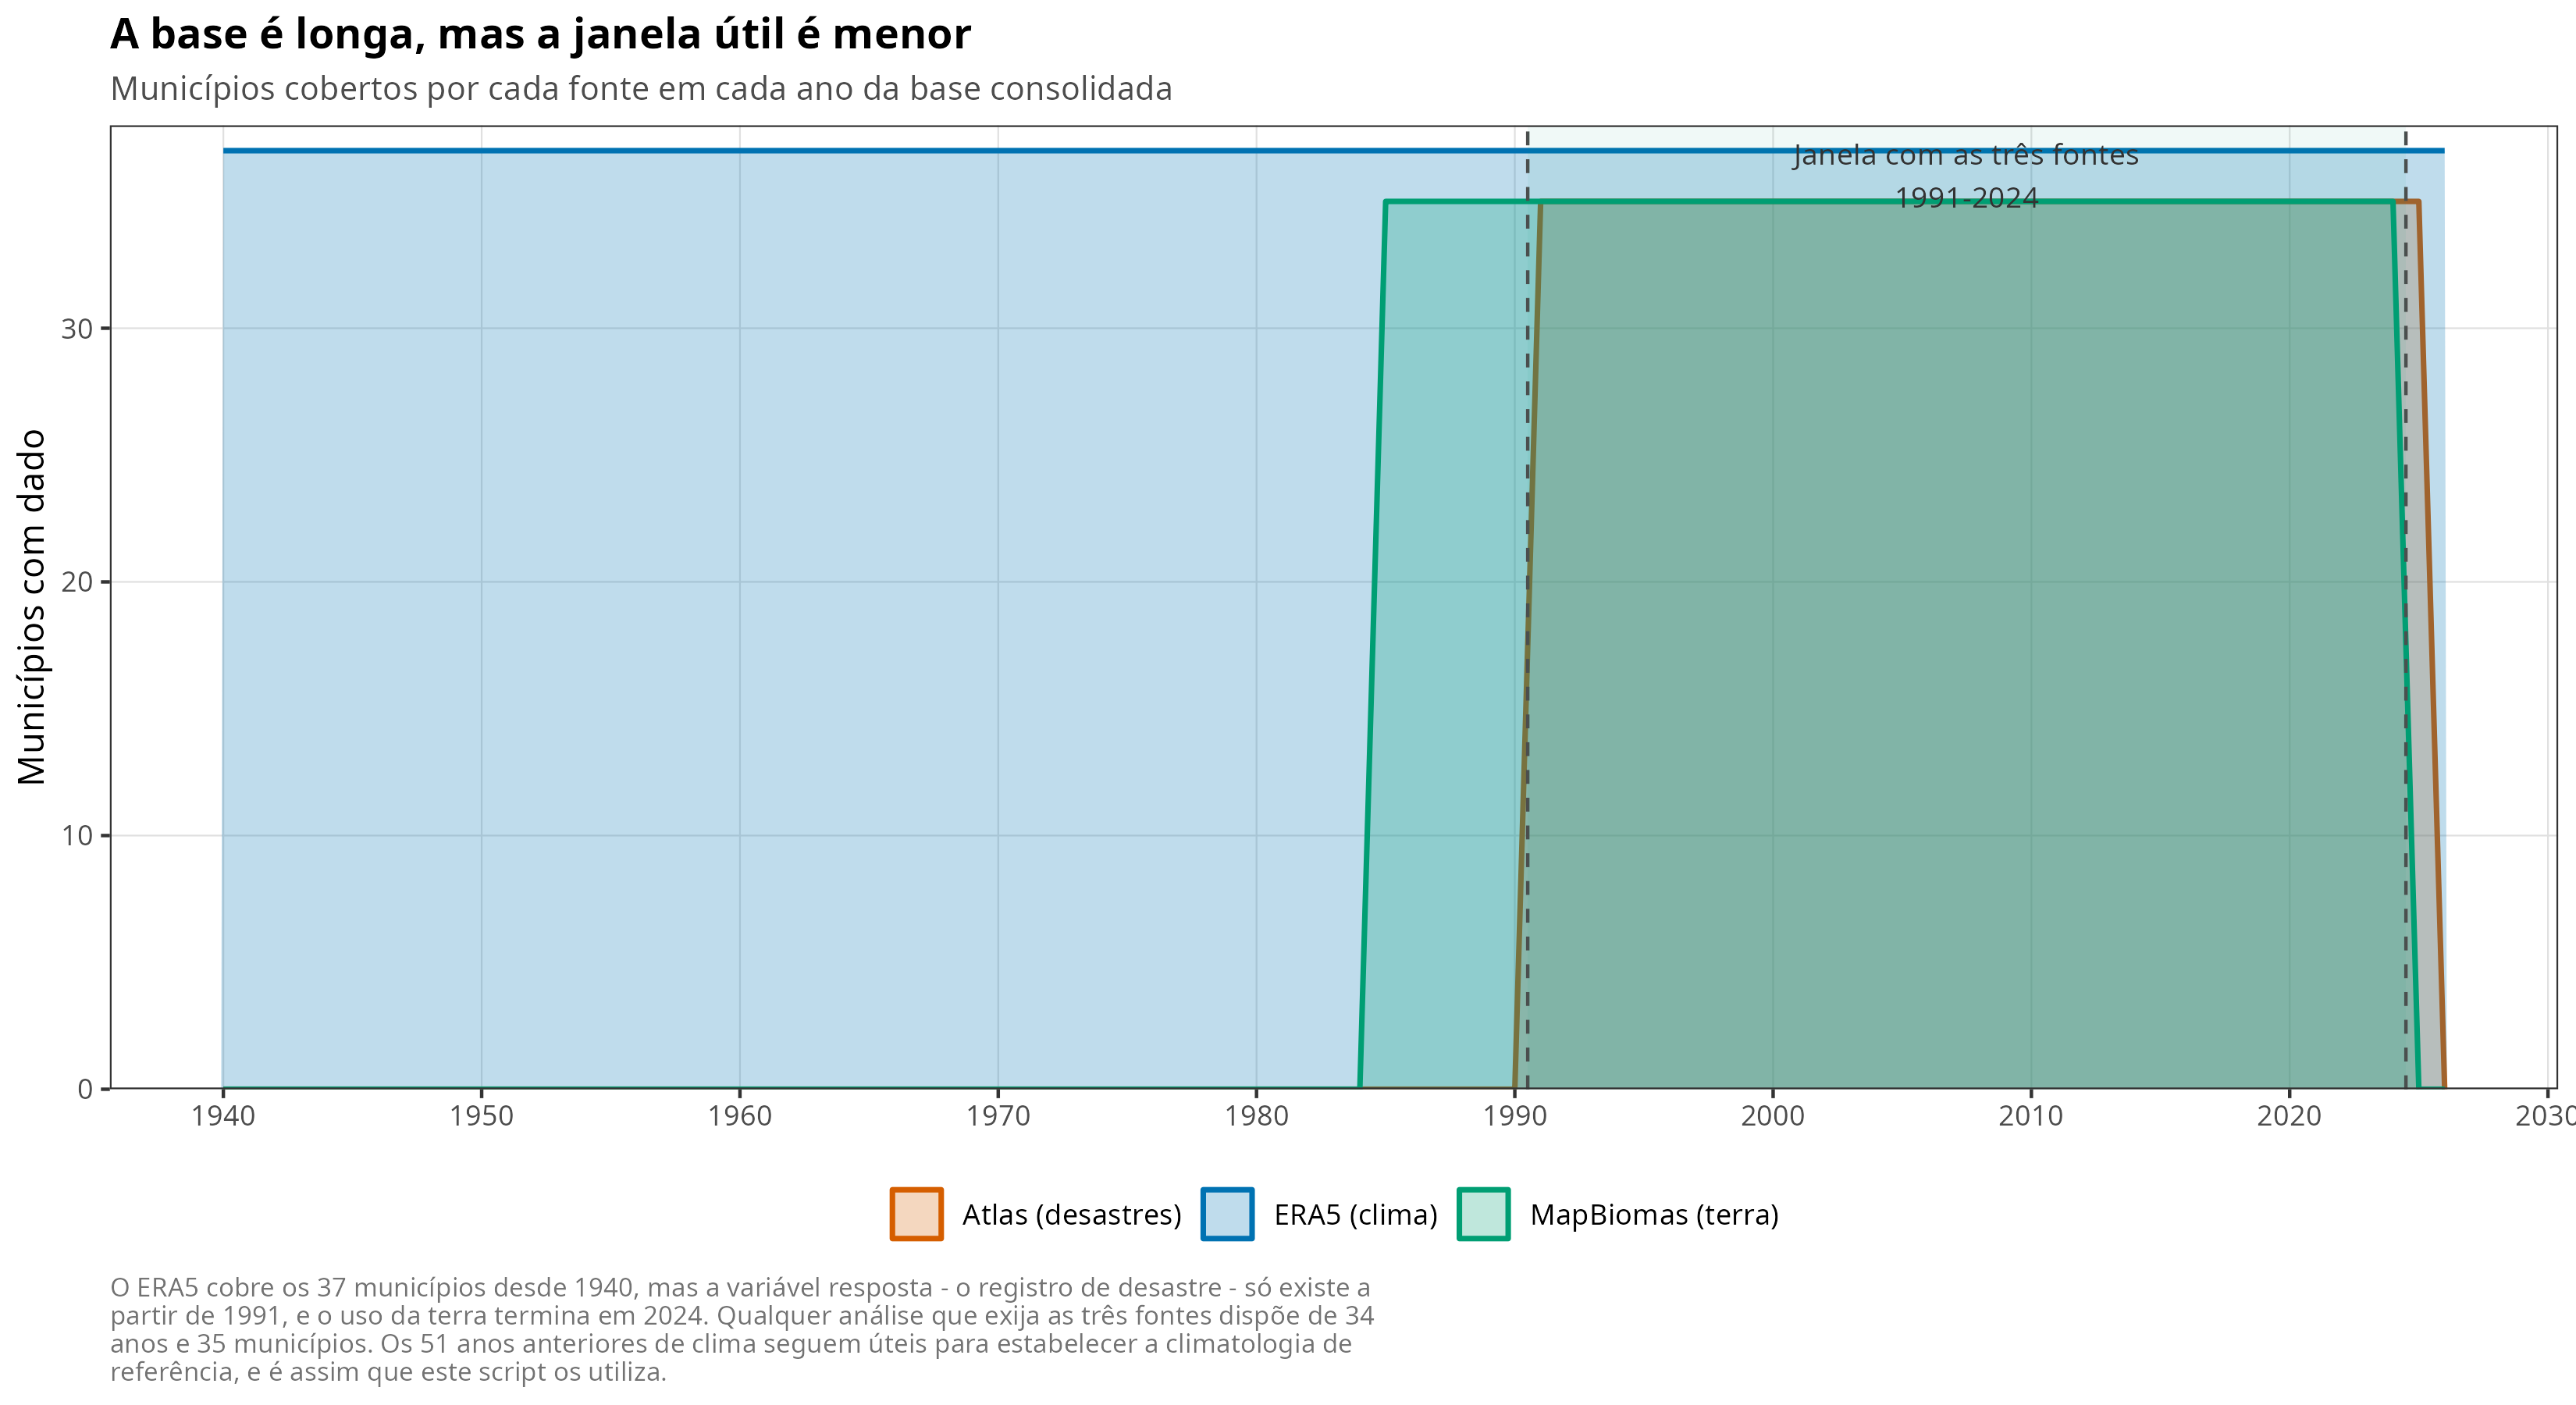
\includegraphics[width=0.95\textwidth]{imagens/aed-A1-janela-util.png}\\[2mm]
{\small Fonte: Elaborado pela autora.}
\end{figure}

Três observações sobre a cobertura. A primeira é que o ERA5 tem grade de 0,25°, o que dá de 1 a 8 pixels por município; Balneário Piçarras, Balneário Arroio do Silva e Passo de Torres têm um único pixel (A03). A segunda é que a superfície de água do MapBiomas cobre só 25 municípios e perde 48\% dos valores na janela, por isso entra apenas como contexto. A terceira é que Camboriú e Paulo Lopes constam no ERA5 e no shapefile (37 municípios), mas não têm registro no Atlas nem valores do MapBiomas na base consolidada; por isso a análise usa 35 municípios. A ausência do MapBiomas nesses dois municípios é suspeita, porque a fonte cobre todo o Brasil, e pode ser falha de junção na consolidação \pendente{verificar o código ou o nome do município na consolidação e a coleção do MapBiomas}.

A base consolidada anterior usava a Climbra, que foi substituída pelo ERA5; a base atual não tem nenhuma variável da Climbra \pendente{registrar o motivo da troca}.

\subsection{Unidades da precipitação do ERA5}

O produto do ERA5 baixado é a reanálise mensal (\textit{monthly averaged reanalysis}), na qual a precipitação total (\texttt{tp}) é a média da acumulação diária, em metros. Como a conversão para milímetros por mês afeta todos os valores de chuva do capítulo, testaram-se três hipóteses (Tabela~\ref{tab:aed-era5}). Só a primeira, multiplicar \texttt{tp} por 1.000 e pelo número de dias do mês, produz um total anual plausível para o litoral catarinense e reproduz a coluna que já existe na base. As razões entre colunas da base confirmam essa conversão: milímetros por dia dividido por \texttt{tp} dá 1.000, e a chuva de larga escala, em kg m$^{-2}$ s$^{-1}$, foi multiplicada por 86.400. O fator 24 só valeria no produto por hora do dia, que não foi usado.

\begin{table}[!htb]
\centering
\caption{Hipóteses de conversão da precipitação do ERA5.}
\label{tab:aed-era5}
{\small
\renewcommand{\arraystretch}{1.2}
\begin{tabular}{@{}p{5.2cm}p{4.6cm}p{3cm}@{}}
\toprule
\textbf{Conversão} & \textbf{Precipitação anual média, 1991--2025 (mm)} & \textbf{Reproduz a coluna da base?}\\
\midrule
\texttt{tp} $\times$ 1.000 $\times$ dias do mês & 1.724 & sim\\
\texttt{tp} $\times$ 1.000 & 57 & não\\
\texttt{tp} $\times$ 1.000 $\times$ 24 $\times$ dias do mês & 41.373 & não\\
\bottomrule
\end{tabular}}\\[2mm]
{\small Fonte: Elaborado pela autora (A04, A05).}
\end{table}

Adotou-se, portanto, a primeira conversão \pendente{confirmar a conversão; dela dependem todos os valores de chuva}. A faixa esperada de 1.300 a 2.000 mm por ano para o litoral de Santa Catarina \pendente{conferir a fonte (INMET) antes de citar} e a comparação do ERA5 com estações do INMET ou da ANA ainda não foram feitas.

% ---------------------------------------------------------------------
\section{Séries temporais por base}
\label{sec:aed-series}

A Figura~\ref{fig:aed-sintese} reúne, no mesmo eixo de tempo, as séries das três bases principais na janela de análise: eventos hidrológicos registrados, precipitação anual média e área urbanizada. A linha tracejada marca 2013, primeiro ano em que a tipologia ``Chuvas Intensas'' aparece no Atlas.

\begin{figure}[!htb]
\centering
\caption{Séries anuais das três bases, 1991--2025. A linha tracejada marca 2013. Cada painel tem sua própria escala.}
\label{fig:aed-sintese}
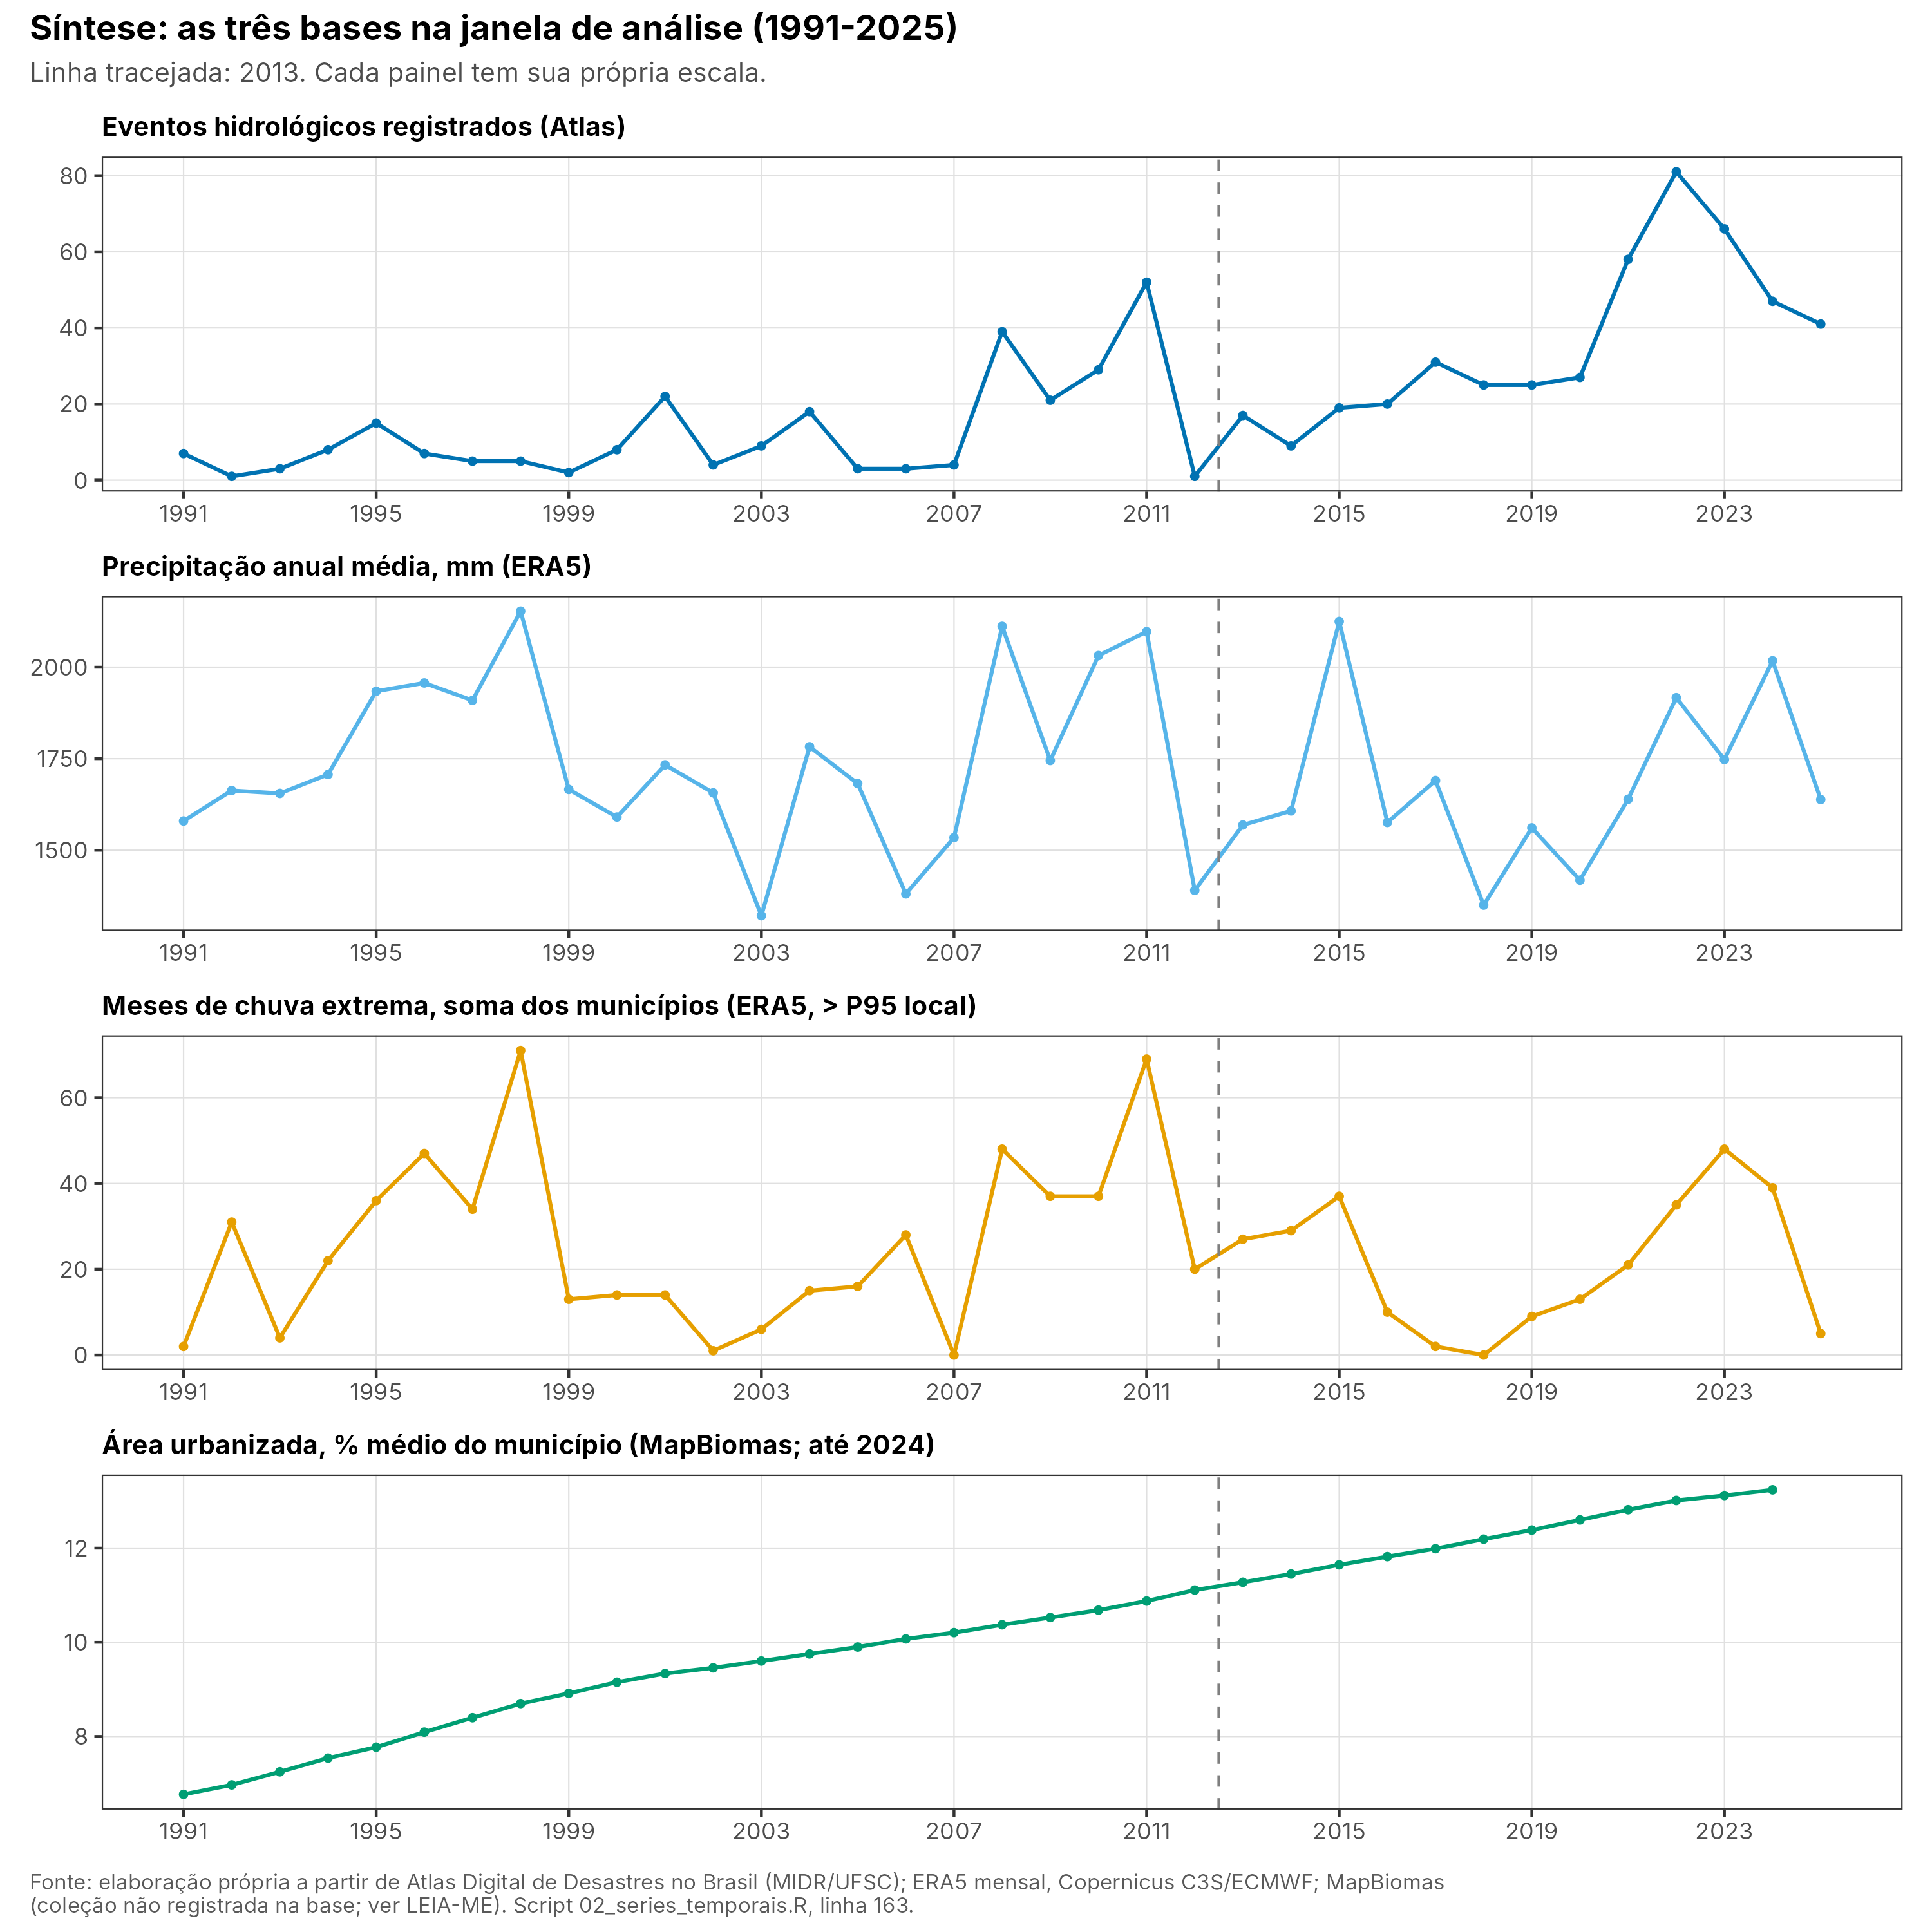
\includegraphics[width=0.85\textwidth]{imagens/aed-B6-sintese-tres-bases.png}\\[2mm]
{\small Fonte: Elaborado pela autora (B07).}
\end{figure}

\paragraph{Atlas Digital de Desastres.} Somando os 35 municípios, o número de eventos hidrológicos passa de uma média de 12,1 por ano em 1991--2012 para 35,8 por ano em 2013--2025, com pico de 81 eventos em 2022 (B01, D01). A série não cresce de modo gradual: há um salto depois de 2013, que coincide com o início do registro de ``Chuvas Intensas'' (Seção~\ref{sec:aed-resposta}). A composição mensal também mudou: janeiro concentra cerca de 20\% dos eventos nos dois períodos (22,2\% em 1991--2012 e 19,3\% em 2013--2025), mas setembro cai de 14,7\% para 3,6\% e junho passa de 0\% para 7,3\% (B05).

\paragraph{ERA5.} A precipitação anual média regional é de 1.724 mm em 1991--2025, variando de 1.327 a 2.158 mm; o maior valor da série completa, de 1940 a 2025, é o de 1983, com 2.509 mm (B02). Janeiro é o mês mais chuvoso, com 220 mm em média, e julho o mais seco, com 99 mm; o maior valor mensal regional ocorre em novembro, com 425 mm (B04). A série anual não mostra tendência (tau de Mann-Kendall de $-0{,}05$), e o número de meses de chuva extrema, definidos como meses acima do percentil 95 local, também não (tau de 0,03) (D02). Vale repetir que isso vale para a chuva mensal da reanálise, que tem resolução de 0,25° e pode não captar extremos diários ou horários.

\paragraph{MapBiomas.} A área urbanizada média dos municípios cresce de modo contínuo, de 6,8\% em 1991 para 13,2\% em 2024, enquanto a floresta cai de 36,6\% para 33,3\% (B06). Como a série termina em 2024, 2025 fica sem valor (2,86\% de ausentes na janela).

% ---------------------------------------------------------------------
\section{Variável resposta: desastres hidrológicos}
\label{sec:aed-resposta}

A variável resposta é o número de eventos do grupo hidrológico registrados no Atlas Digital de Desastres, por município e por ano. No período 1991--2025 há 732 eventos, em cinco tipologias (C01, C02): Chuvas Intensas (289 eventos, 39,5\%), Enxurradas (277, 37,8\%), Alagamentos (73), Inundações (69) e Movimento de massa (24). Como a tipologia ``Chuvas Intensas'' só existe a partir de 2013, a resposta pode ser lida de três modos: o total (732 eventos), o total sem Chuvas Intensas (443 eventos, 60,5\%) e só Chuvas Intensas (289 eventos, 39,5\%). Esse grupo, tal como aparece na base consolidada, é mais amplo que o grupo Hidrológico da classificação oficial (COBRADE): nela, só inundações (1.2.1), enxurradas (1.2.2) e alagamentos (1.2.3) são hidrológicos, os movimentos de massa são geológicos (1.1.3) e as chuvas intensas são meteorológicas (1.3.2.1.4). A resposta deste trabalho é, portanto, um agrupamento operacional \pendente{confirmar se esse agrupamento vem do Atlas ou da etapa de consolidação, e citar a Instrução Normativa MI nº 1/2012}. Esse detalhe decide o que se pode afirmar, e por isso as três versões são mantidas lado a lado neste capítulo \pendente{decidir qual versão da resposta segue para a modelagem}.

\subsection{Composição no tempo}

Enxurradas eram 96,9\% dos eventos em 2006--2010 e passam a 5,8\% em 2021--2025, enquanto Chuvas Intensas chegam a 77,8\% dos eventos nesse último bloco (C03; Figuras~\ref{fig:aed-composicao} e~\ref{fig:aed-tipologias}). Ou seja, a mudança de composição é tão forte quanto a mudança de volume. Qualquer afirmação sobre ``aumento dos desastres'' precisa dizer de qual versão da resposta fala: com o total, há forte tendência de alta (tau de Mann-Kendall de 0,53 em 1991--2025); sem Chuvas Intensas, a razão entre a média anual depois e antes de 2013 é de apenas 1,13 (D01, D02).

\begin{figure}[!htb]
\centering
\caption{Composição do grupo hidrológico por bloco de cinco anos, nos 35 municípios.}
\label{fig:aed-composicao}
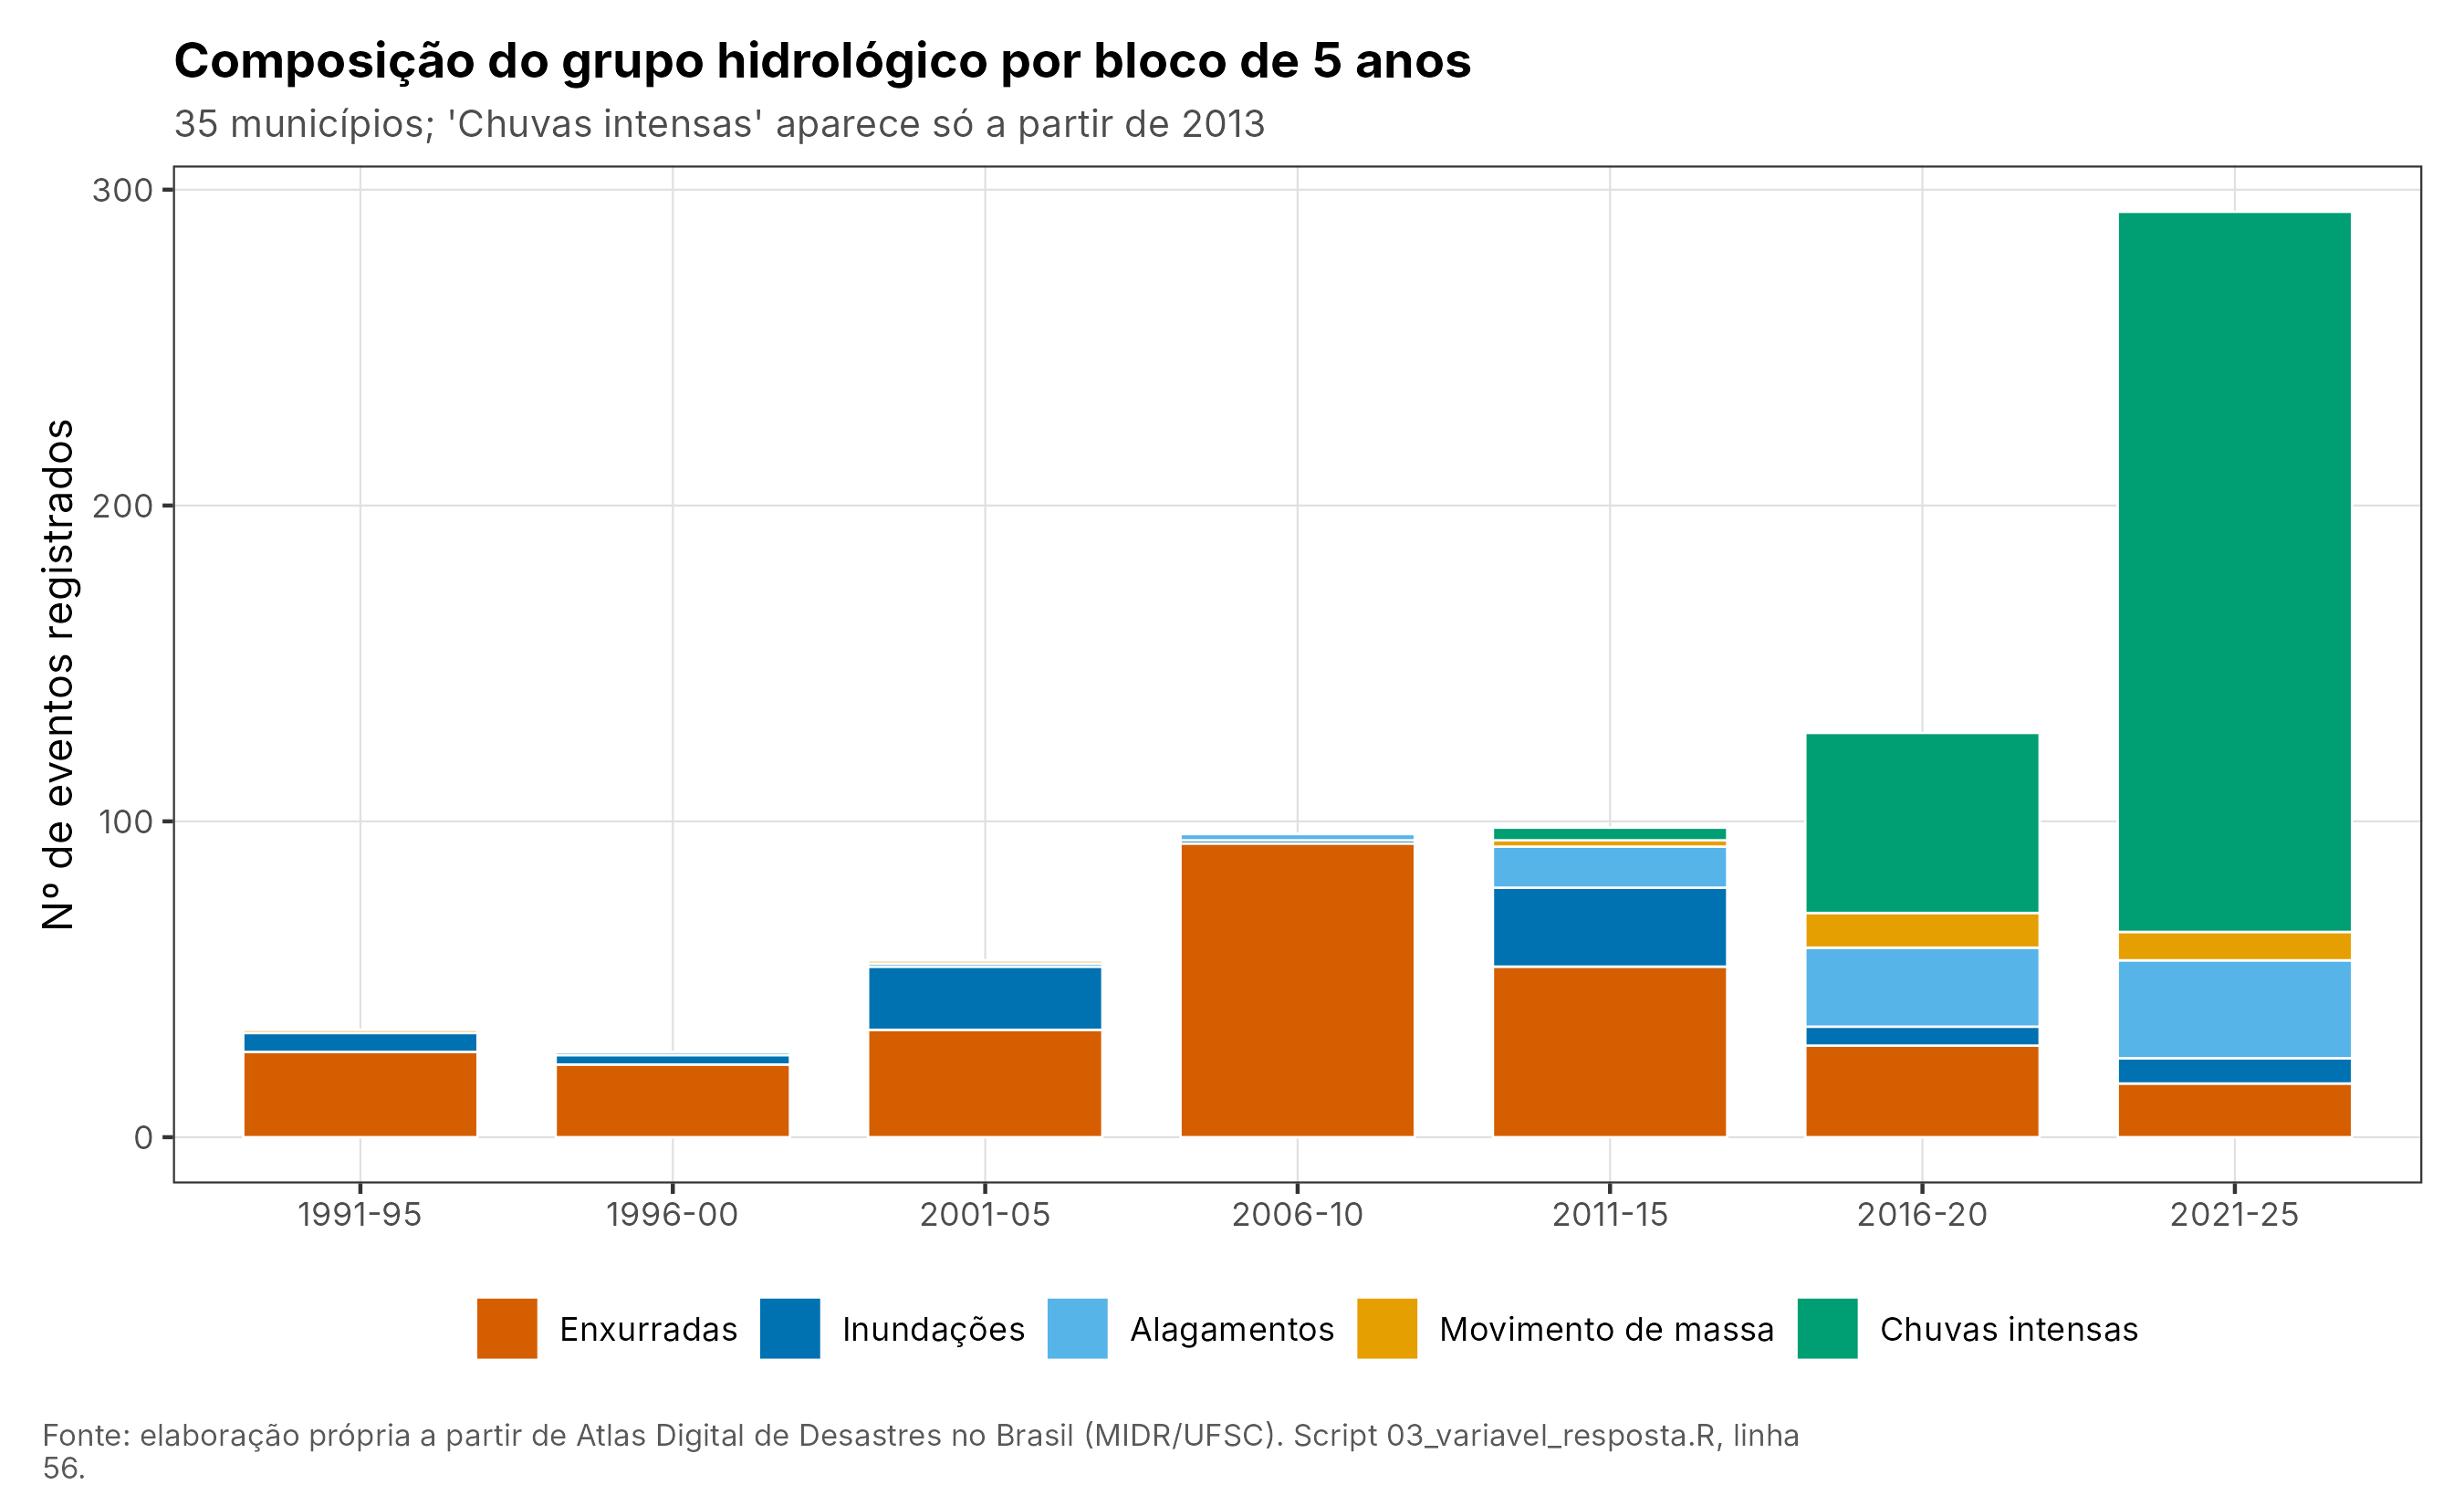
\includegraphics[width=0.8\textwidth]{imagens/aed-C1-composicao-blocos.png}\\[2mm]
{\small Fonte: Elaborado pela autora (C03).}
\end{figure}

\begin{figure}[!htb]
\centering
\caption{Eventos por tipologia e por ano. A linha tracejada marca 2013.}
\label{fig:aed-tipologias}
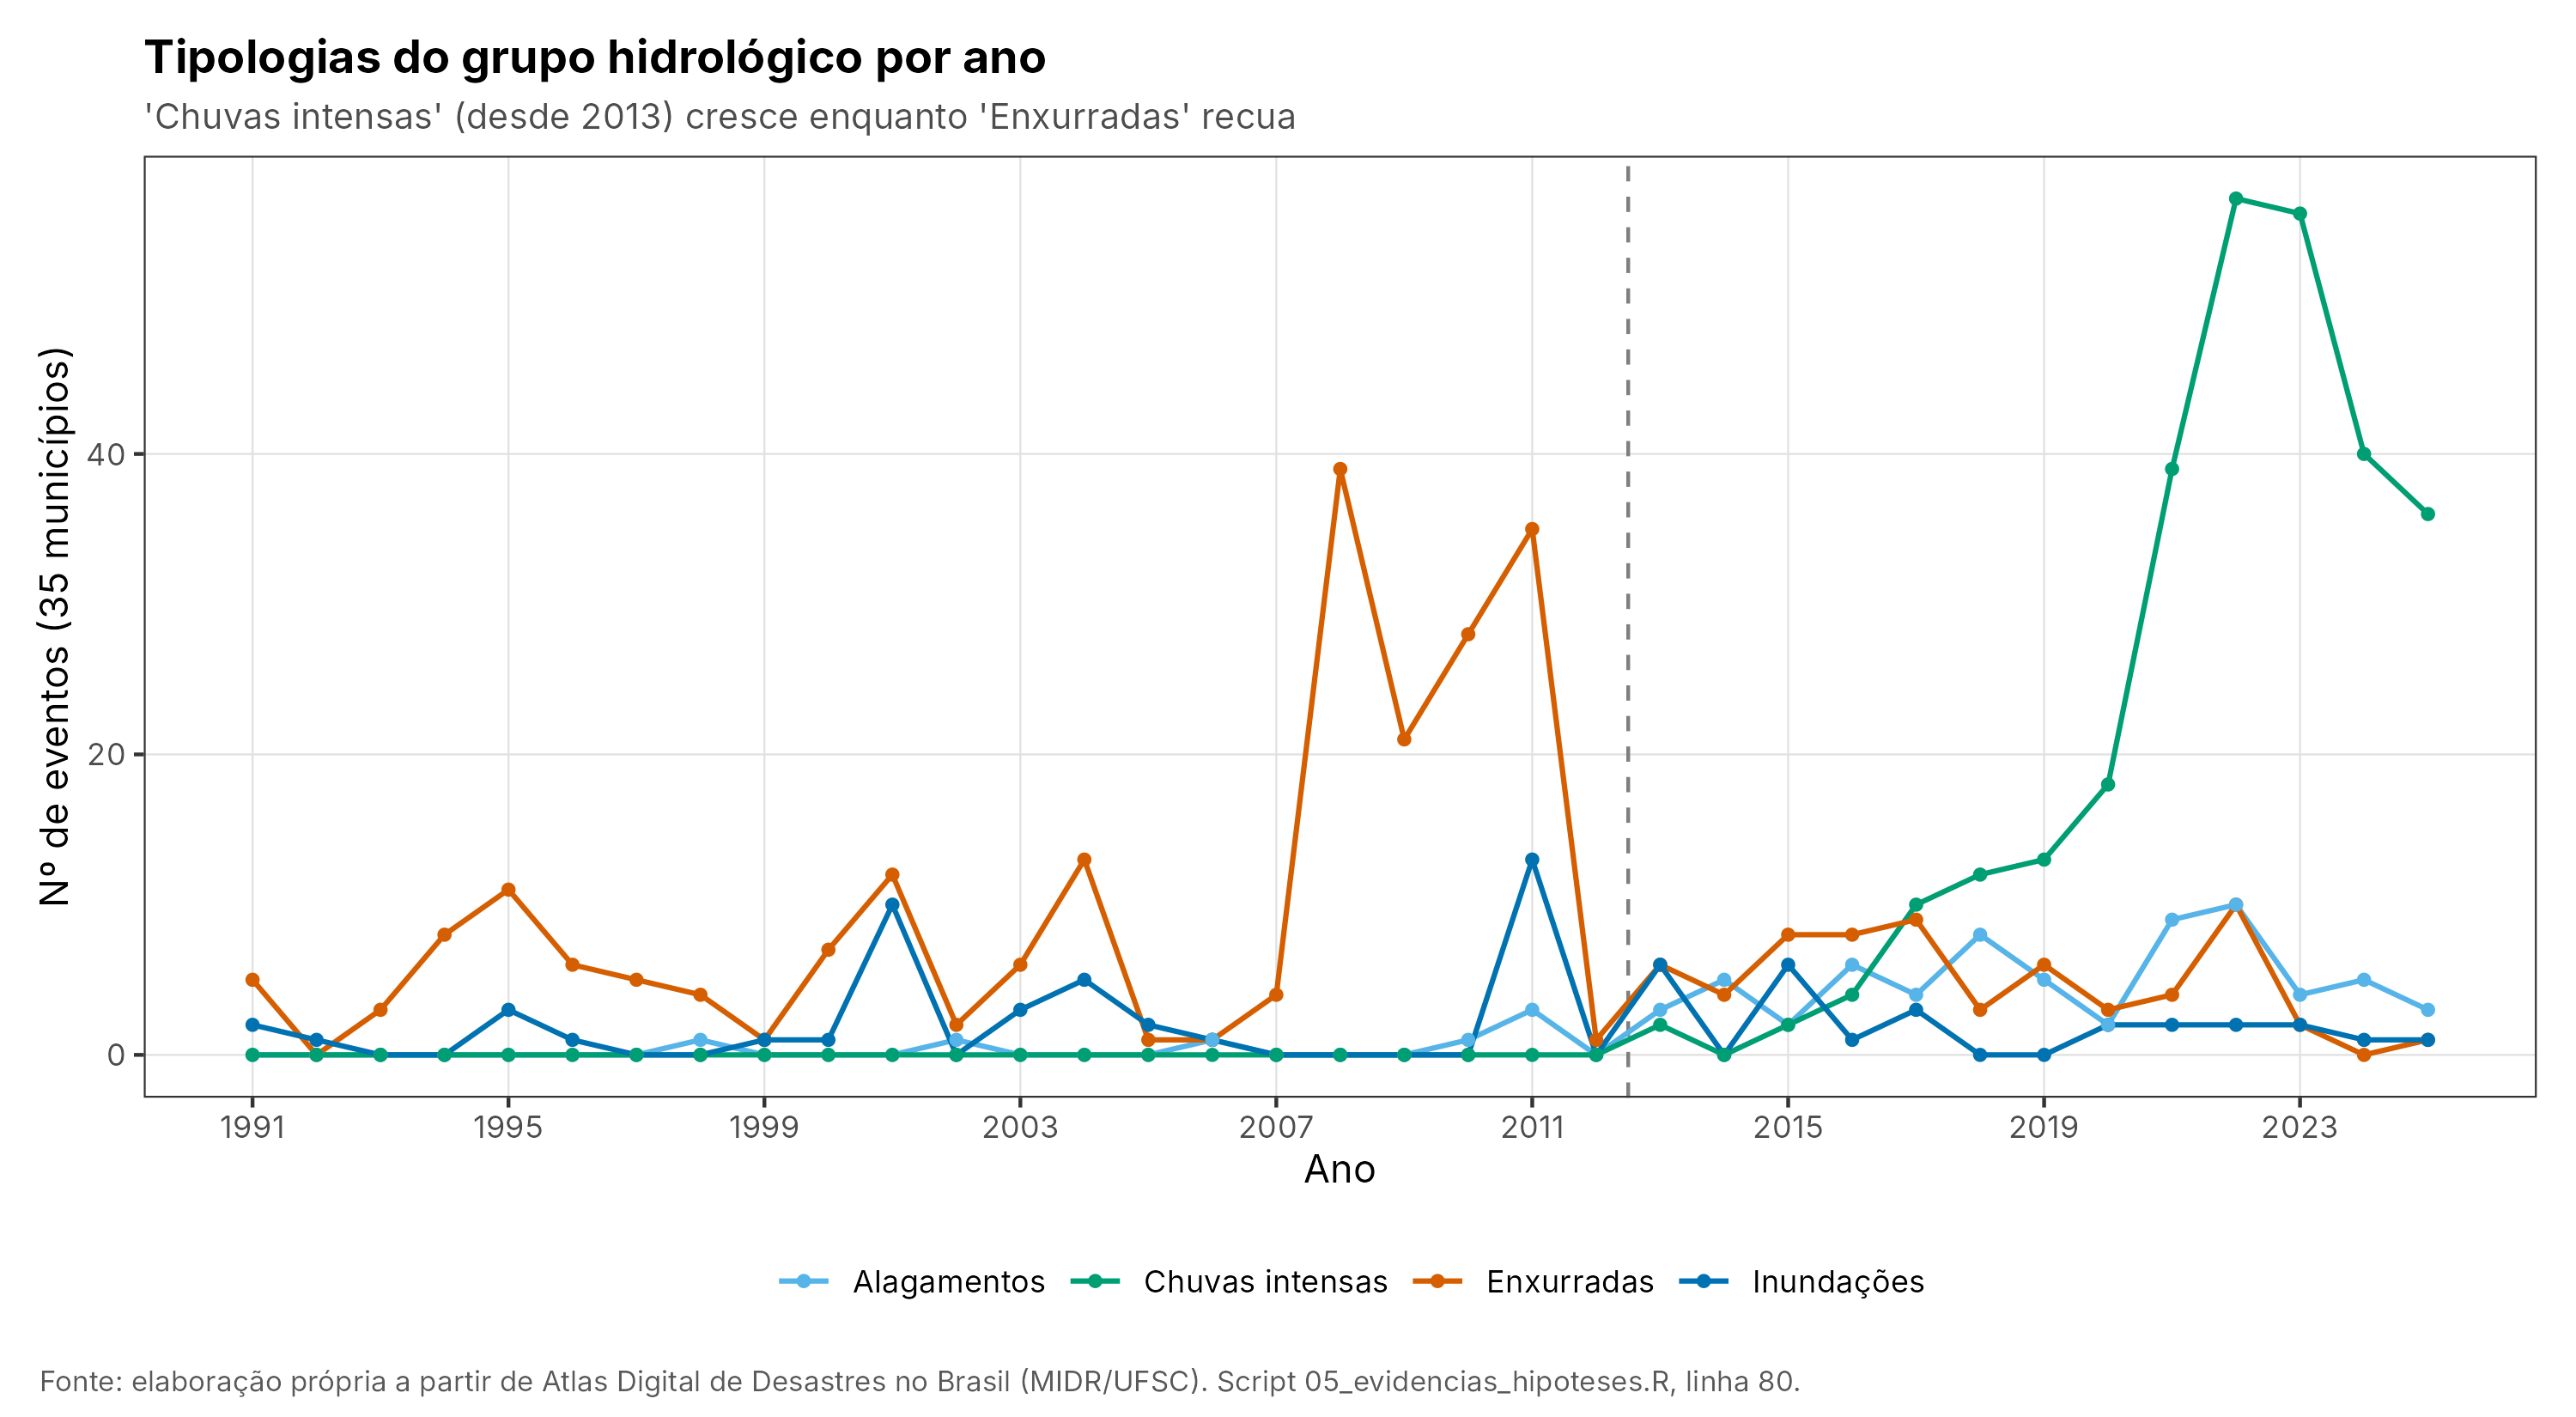
\includegraphics[width=0.8\textwidth]{imagens/aed-D1-enxurradas-chuvas-intensas.png}\\[2mm]
{\small Fonte: Elaborado pela autora (D03).}
\end{figure}

\subsection{Distribuição por município e por ano}

No nível do município-ano (1.225 observações, 35 municípios por 35 anos), a média é de 0,60 evento e o máximo é 7. Em 62,8\% dos município-anos não há registro de evento; essa proporção é de 72,6\% sem Chuvas Intensas e de 86,3\% só com Chuvas Intensas (C04, C05; Figura~\ref{fig:aed-contagens}). A razão entre variância e média é de 1,67 no município-ano, mas de 19,5 na série anual agregada, o que mostra que os registros se agrupam em poucos anos e municípios. Essa razão é uma descrição da dispersão, e não um modelo.

\begin{figure}[!htb]
\centering
\caption{Distribuição do número de eventos por município-ano, nas três versões da resposta.}
\label{fig:aed-contagens}
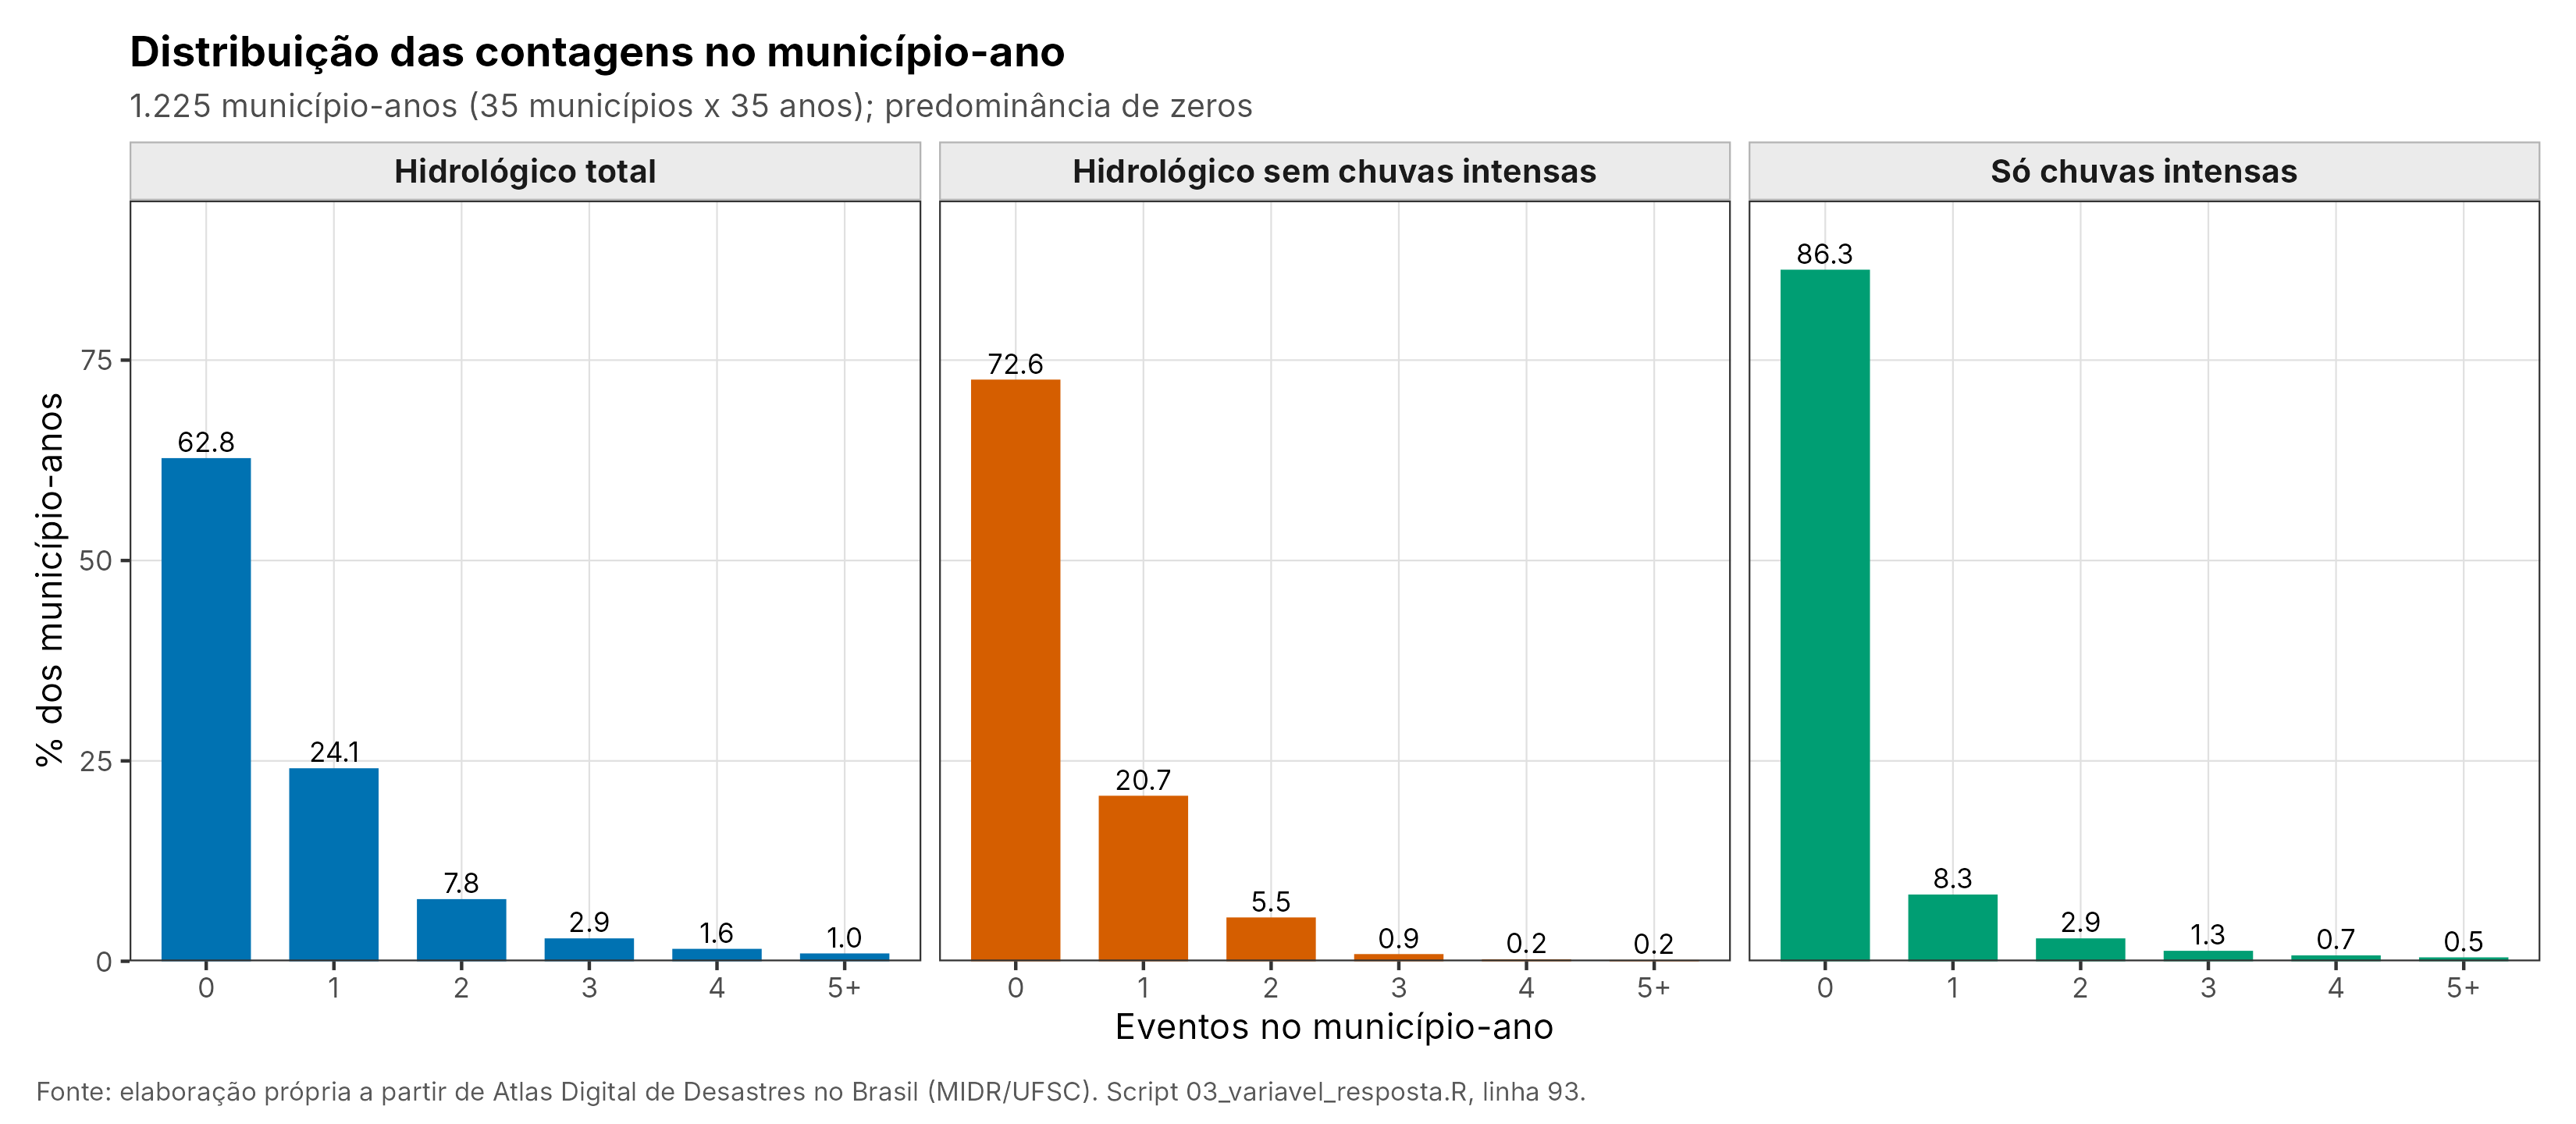
\includegraphics[width=0.85\textwidth]{imagens/aed-C2-distribuicao-contagens.png}\\[2mm]
{\small Fonte: Elaborado pela autora (C05).}
\end{figure}

Entre os municípios, a mediana é de 19 eventos, com mínimo de 6 e máximo de 46. Joinville (46), Florianópolis (38) e Balneário Camboriú (33) lideram em número absoluto (Figura~\ref{fig:aed-municipios}); em densidade, Balneário Camboriú tem 721 eventos por mil km$^{2}$ (C07). Os dois municípios sem Atlas, Camboriú e Paulo Lopes, têm 100\% de valores ausentes na resposta e não entram como zeros (C06).

\begin{figure}[!htb]
\centering
\caption{Eventos hidrológicos por município, 1991--2025.}
\label{fig:aed-municipios}
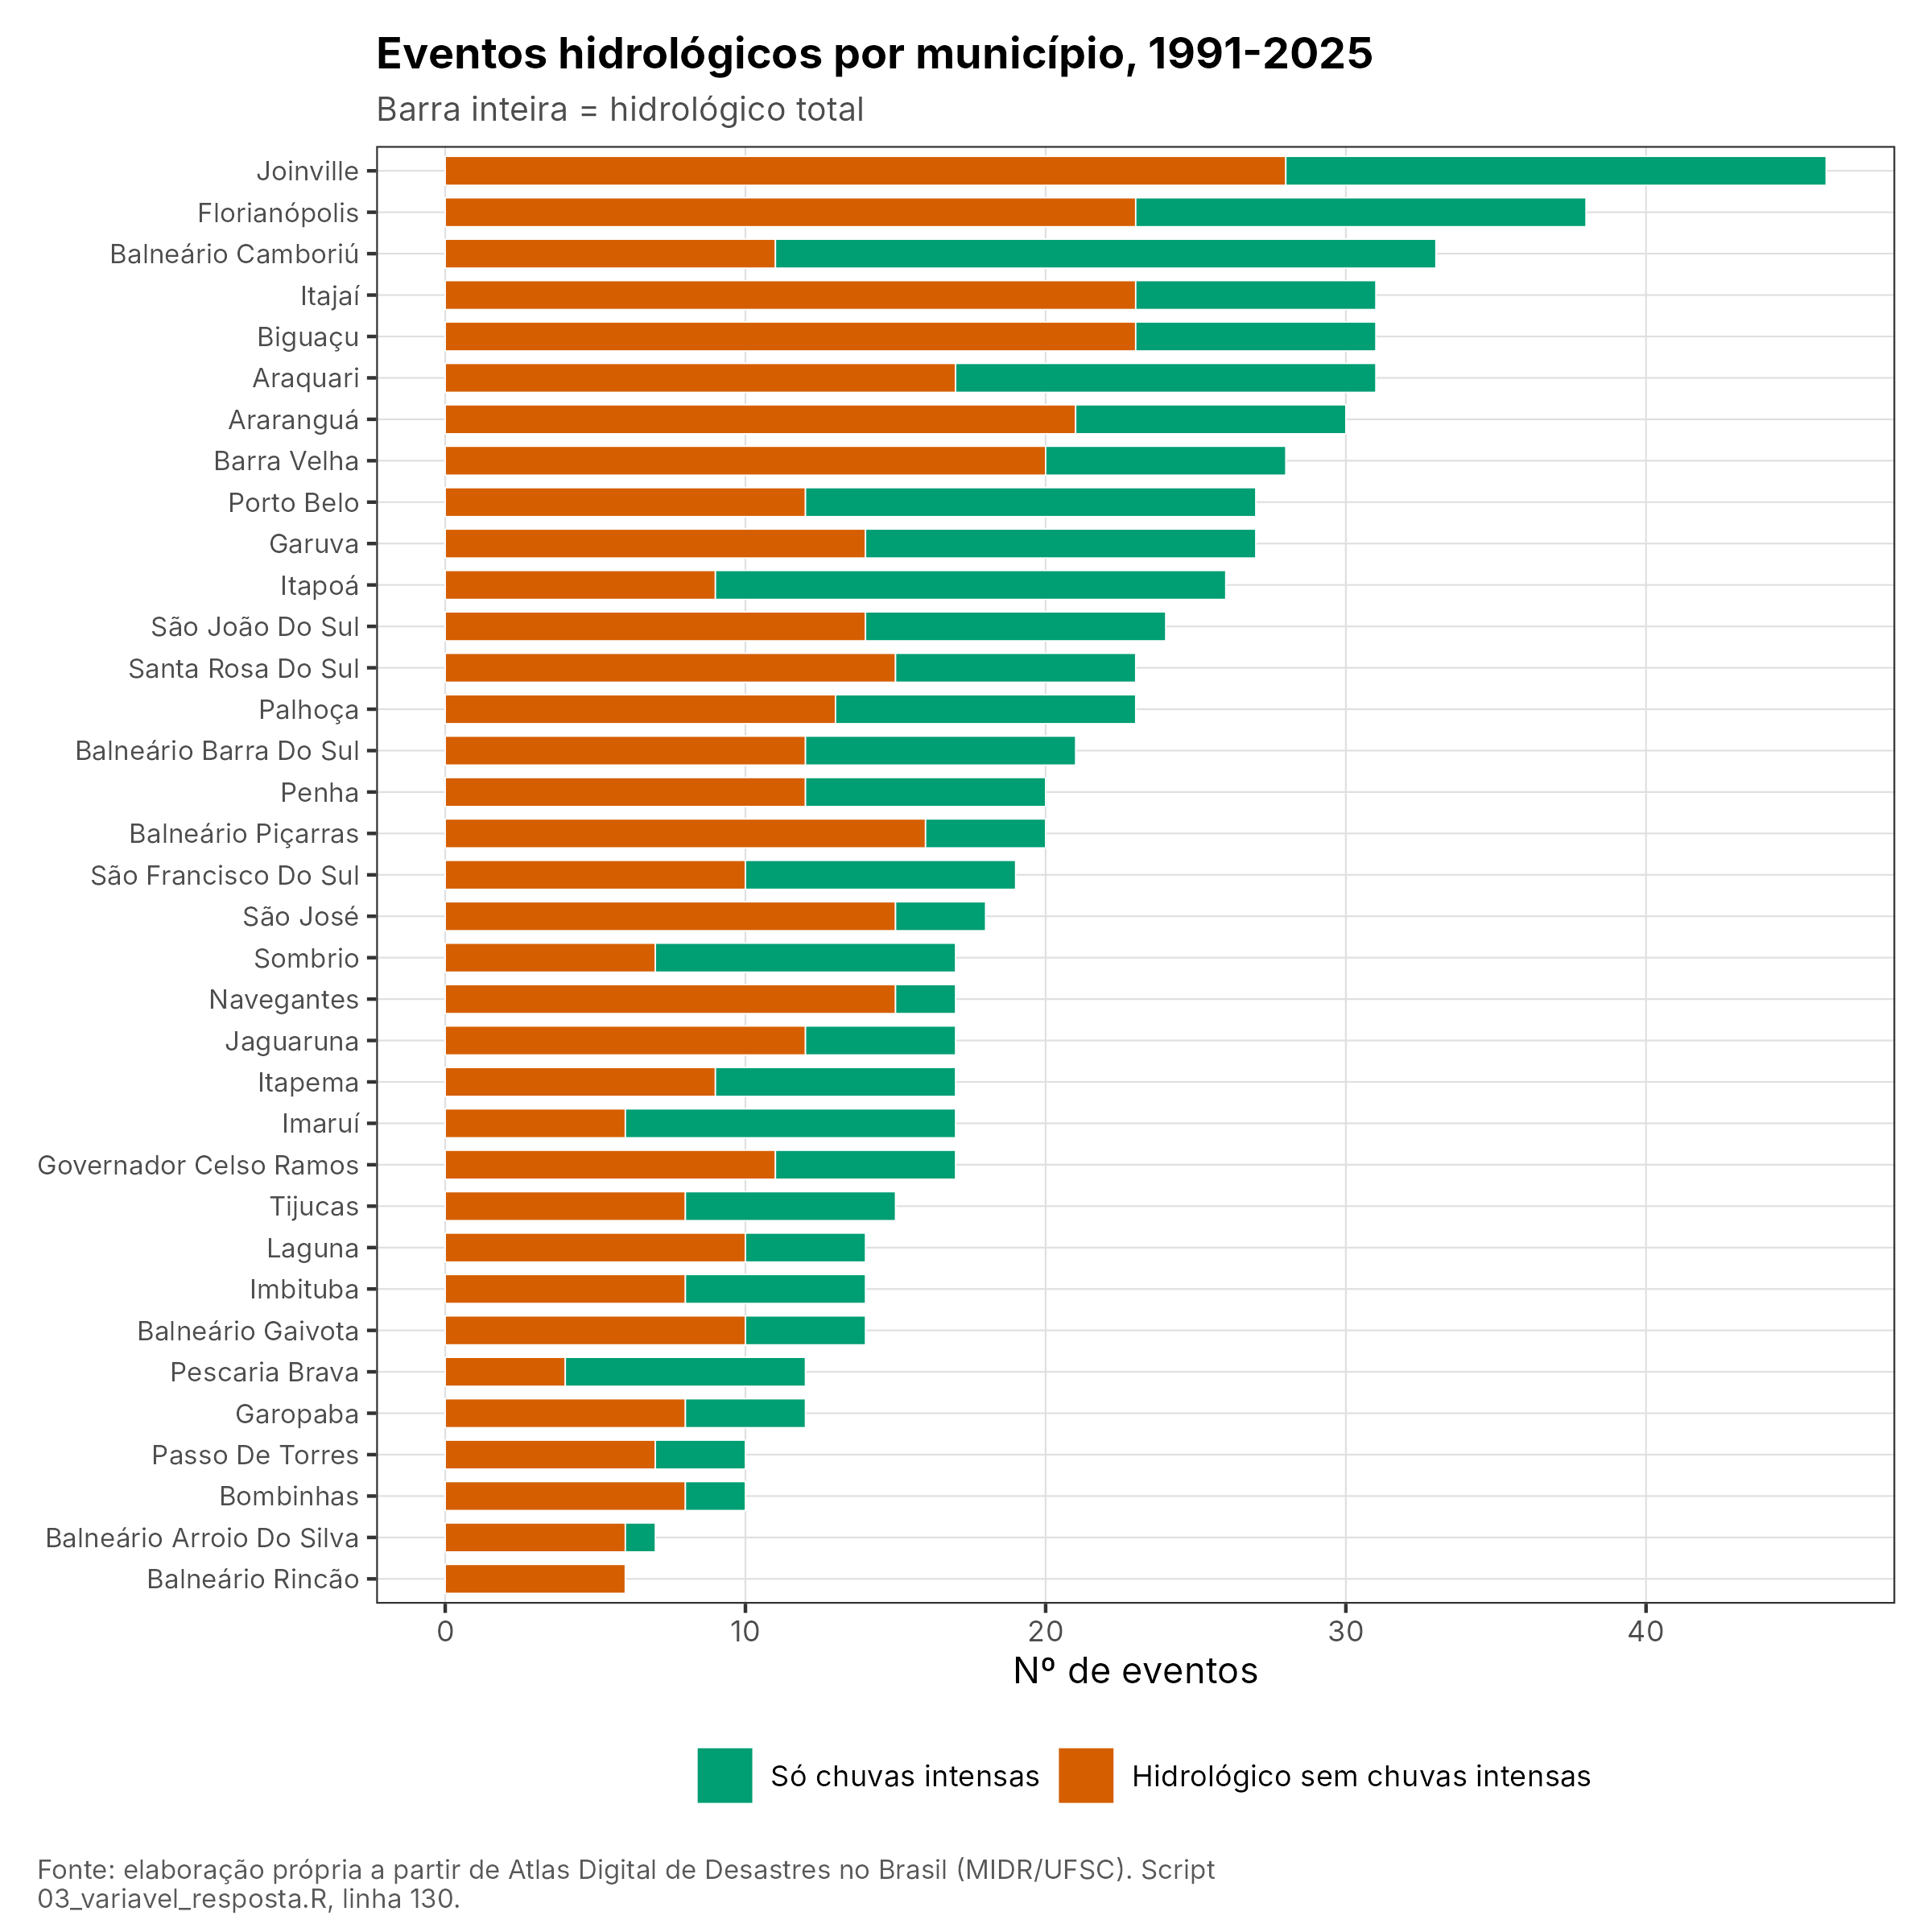
\includegraphics[width=0.7\textwidth]{imagens/aed-C3-eventos-por-municipio.png}\\[2mm]
{\small Fonte: Elaborado pela autora (C07).}
\end{figure}

% ---------------------------------------------------------------------
\section{Variáveis preditoras}
\label{sec:aed-preditoras}

As variáveis candidatas a explicar a resposta vêm do ERA5 (chuva e vento) e do MapBiomas (uso da terra e áreas de risco). A Tabela~\ref{tab:aed-preditoras} traz a média no município-ano, os valores ausentes e uma medida que importa para a modelagem: que parte da variação ocorre entre municípios e que parte ocorre ao longo do tempo.

\begin{table}[!htb]
\centering
\caption{Variáveis preditoras: descrição no município-ano.}
\label{tab:aed-preditoras}
{\small
\renewcommand{\arraystretch}{1.2}
\begin{tabular}{@{}p{5cm}p{3.2cm}p{1.8cm}p{3.4cm}@{}}
\toprule
\textbf{Variável} & \textbf{Média (município-ano)} & \textbf{Ausentes} & \textbf{\% da variação entre municípios}\\
\midrule
Precipitação anual (mm) & 1.718 (dp 342) & 0\% & 44,5\%\\
Maior acumulado de 3 meses (mm) & 654 & 0\% & 40,4\%\\
Meses de chuva extrema (0--12) & 0,69 & 0\% & 0\% (por construção: percentil local)\\
Vento a 10 m (m/s) & 3,02 & 0\% & 98,7\%\\
Área urbanizada (\%) & 10,3 & 2,86\% & 92,4\%\\
Floresta (\%) & 34,5 & 2,86\% & 99,2\%\\
Área urbana em risco (ha) & 186 & 6,29\% & 99,4\%\\
\bottomrule
\end{tabular}}\\[2mm]
{\small Fonte: Elaborado pela autora (C09, C10).}
\end{table}

O uso da terra varia quase só entre municípios, enquanto a chuva varia tanto no espaço quanto no tempo. Isso limita o que o MapBiomas pode dizer sobre a tendência dos desastres ao longo do tempo: ele descreve diferenças entre lugares, e não mudanças no mesmo lugar.

Algumas preditoras são redundantes entre si. Os pares com correlação de Spearman de módulo maior ou igual a 0,7 são área urbanizada e área não vegetada (0,97), maior acumulado de 3 meses e chuva anual (0,84), vento e chuva convectiva ($-0{,}75$), floresta e nuvens (0,76) e floresta e vento ($-0{,}71$) (C11, C12). Esses pares não devem entrar juntos em uma etapa posterior sem tratamento.

O papel de cada variável na análise (resposta, preditora, controle, exposição ou contexto) é uma proposta e consta na coluna correspondente da tabela de metadados do repositório (A02) \pendente{revisar a coluna ``papel'' de A02}.

% ---------------------------------------------------------------------
\section{Hipóteses sobre a coleta dos dados e sobre outros fatores}
\label{sec:aed-hipoteses}

A série de desastres mede ao mesmo tempo o clima e a forma como os desastres são registrados. Esta seção reúne evidências para duas hipóteses e trata ambas como hipóteses abertas: a hipótese H1, de que parte do aumento dos registros decorre de mudanças na coleta e na classificação; e a hipótese H2, de que fatores além da chuva, como o uso da terra e a posição geográfica, contribuem para a distribuição dos eventos. Nenhuma linha da Tabela~\ref{tab:aed-evidencias} isola uma causa; cada uma tem uma leitura alternativa no quadro de evidências do repositório (D00).

\begin{table}[!htb]
\centering
\caption{Evidências para as hipóteses de coleta (H1) e de outros fatores (H2).}
\label{tab:aed-evidencias}
{\small
\renewcommand{\arraystretch}{1.2}
\begin{tabular}{@{}p{1.6cm}p{4.2cm}p{7.2cm}@{}}
\toprule
\textbf{Hipótese} & \textbf{Evidência} & \textbf{Valor}\\
\midrule
H1 & Quebra de 2013 & o total sobe 2,96 vezes depois de 2013; sem Chuvas Intensas, só 1,13 vez (D01)\\
H1 & Enxurradas e Chuvas Intensas & enxurradas passam de 96,9\% para 5,8\% do total; tau de Mann-Kendall de 2013 a 2025 de $-0{,}39$ (p 0,075) (C03, D02)\\
H1 & Eventos sobem, chuva não & Spearman entre eventos e ano 0,73; entre meses extremos e ano 0,02; tau da chuva anual $-0{,}05$ (D04, D02)\\
H1 & Mais municípios registram & 9,4 municípios por ano em 1991--2012 contra 19,2 em 2013--2025 (D07)\\
H1 & Reconhecimento federal (todos os grupos) & 81\% dos eventos em 2009--2011 e 20\% em 2021--2025 (D07)\\
H1 e H2 & Sinal da chuva no alvo sem Chuvas Intensas & razão P(evento) entre a maior e a menor classe de chuva anual: 3,80 em 1991--2012 e 1,38 em 2013--2025 (D06)\\
Controle & Vento também discrimina antes de 2013 & razão 2,43 em 1991--2012 e 1,07 depois; vento e chuva convectiva, rho $-0{,}75$ (D06, C11)\\
H2 & Padrão espacial (I de Moran, 4 vizinhos) & densidade total 0,37 (p 0,001); sem Chuvas Intensas 0,53; só Chuvas Intensas 0,17; percentual de Chuvas Intensas 0,10, sem padrão detectável (D10)\\
H2 & Uso da terra entre municípios (n = 35, bruto) & floresta 0,47 (floresta e latitude 0,78); área urbanizada $-0{,}08$; área urbana em risco 0,30 (D09)\\
\bottomrule
\end{tabular}}\\[2mm]
{\small Fonte: Elaborado pela autora (D00).}
\end{table}

\subsection{H1: a coleta e a classificação mudaram}

As evidências são compatíveis com uma mudança no registro em torno de 2013, mas não a provam. O total de eventos sobe cerca de três vezes depois de 2013, mas a chuva média fica estável (razão de 0,97) e os meses de chuva extrema caem (razão de 0,82) (D01). Sem Chuvas Intensas, a série praticamente não muda (razão de 1,13), e as Enxurradas recuam enquanto as Chuvas Intensas aparecem (Figura~\ref{fig:aed-tipologias}). Além disso, mais municípios passam a registrar eventos a cada ano, e o percentual de eventos com reconhecimento federal cai de 81\% para 20\% (D07).

Duas ressalvas pesam nessa leitura. A primeira é que o indicador de reconhecimento mistura todos os grupos de desastre, e em 2009 100\% dos eventos aparecem como reconhecidos, o que pode ser um artefato. A segunda é que mais municípios atingidos também ocorreria com mais eventos de fato; por isso as evidências de coleta são indícios, e não medidas. Se os registros de Chuvas Intensas substituem tipologias antigas, o aumento do total seria em parte uma mudança de rótulo; essa pergunta depende de uma nota técnica sobre a classificação, que não foi localizada \pendente{verificar se há nota técnica da Defesa Civil ou da COBRADE sobre a classificação adotada em 2012--2013}.

O corte em 2013, primeiro ano com Chuvas Intensas, é o adotado neste capítulo; o corte em 2012, usado na análise exploratória original, dá resultados parecidos (razão do total de 2,64 e, sem Chuvas Intensas, de 1,01) e consta em D01 \pendente{confirmar o corte}.

\subsection{Dose-resposta e controle negativo}

A Figura~\ref{fig:aed-dose} compara a proporção de município-anos com ao menos um evento entre classes de cada descritor climático. Na versão sem Chuvas Intensas, o sinal da chuva anual é forte antes de 2013 (razão de 3,80 entre a maior e a menor classe) e quase desaparece depois (1,38). Isso é compatível com a ideia de que os eventos mais sensíveis à chuva migraram para a nova tipologia, mas também com outras explicações, e por isso a separação da resposta muda a leitura do clima.

O vento foi incluído como controle negativo: uma variável sem relação causal esperada com os eventos, usada para testar se qualquer variável climática ``discrimina'' os registros. O resultado não é limpo. O vento também discrimina antes de 2013 (razão de 2,43) e deixa de discriminar depois (1,07), e ele covaria com a chuva convectiva (rho de $-0{,}75$), porque sistemas frontais e ciclones trazem vento e chuva juntos. O vento serve, assim, como alerta, e não como prova de que o efeito da chuva é específico \pendente{manter o vento como controle negativo ou trocar por outra variável que não covarie com a chuva}.

\begin{figure}[!htb]
\centering
\caption{Proporção de município-anos com ao menos um evento, por classe do descritor, em 1991--2012 (tracejado) e 2013--2025 (contínuo). O vento é o controle negativo.}
\label{fig:aed-dose}
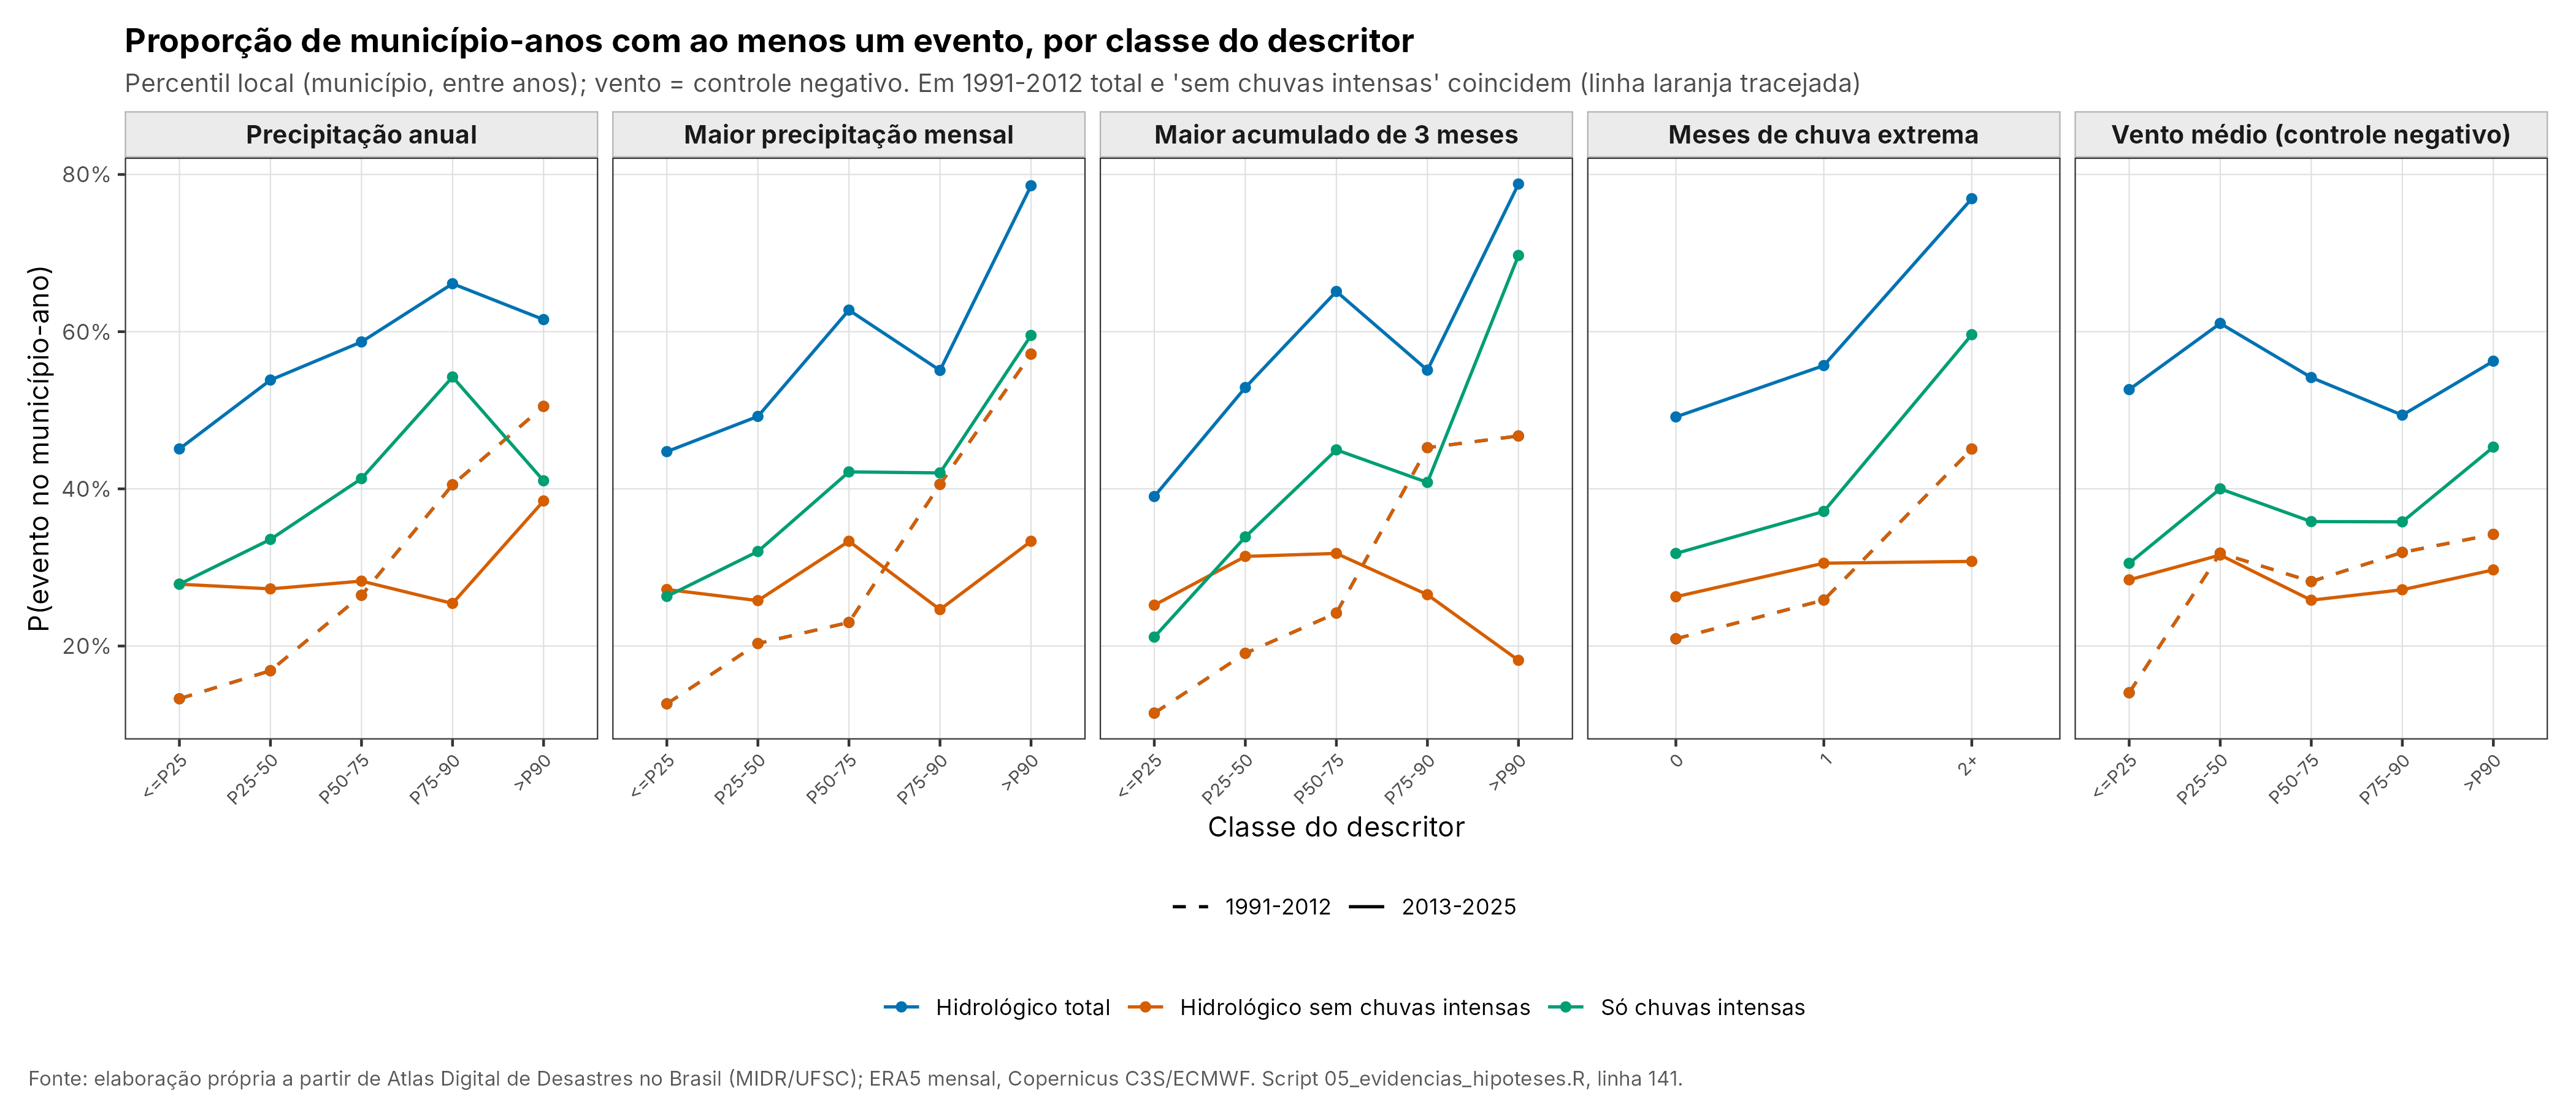
\includegraphics[width=\textwidth]{imagens/aed-D2-dose-resposta-controle-negativo.png}\\[2mm]
{\small Fonte: Elaborado pela autora (D05, D06).}
\end{figure}

\subsection{H2: outros fatores além da chuva}

O padrão espacial dos eventos é descrito pelo índice de Moran, calculado com os quatro vizinhos mais próximos de cada município e 999 permutações (semente 42). A densidade de eventos por mil km$^{2}$ mostra valores parecidos entre vizinhos (0,37 no total e 0,53 sem Chuvas Intensas), assim como a precipitação média (0,50) e o percentual urbanizado (0,30); o percentual de Chuvas Intensas, ao contrário, não mostra padrão espacial detectável (0,10) (D10; Figura~\ref{fig:aed-mapas}). O índice descreve, mas não explica: o agrupamento pode vir do clima regional, das bacias hidrográficas ou da prática de registro de uma mesma regional da Defesa Civil.

Entre municípios, a correlação bruta dos eventos totais com a floresta é de 0,47, mas a floresta acompanha a latitude (0,78), assim como o vento e outras variáveis, no eixo norte--sul; a associação com os eventos pode refletir apenas esse gradiente. A área urbanizada praticamente não se associa aos eventos ($-0{,}08$), a área urbana em risco tem associação moderada (0,30) e a latitude tem associação de 0,49, com mais eventos ao norte (D09). Com 35 municípios e sem modelagem, esses números são associações brutas, e cada descritor é apresentado junto com sua correlação com a latitude.

\begin{figure}[!htb]
\centering
\caption{Mapas da densidade de eventos e da composição da resposta, por município.}
\label{fig:aed-mapas}
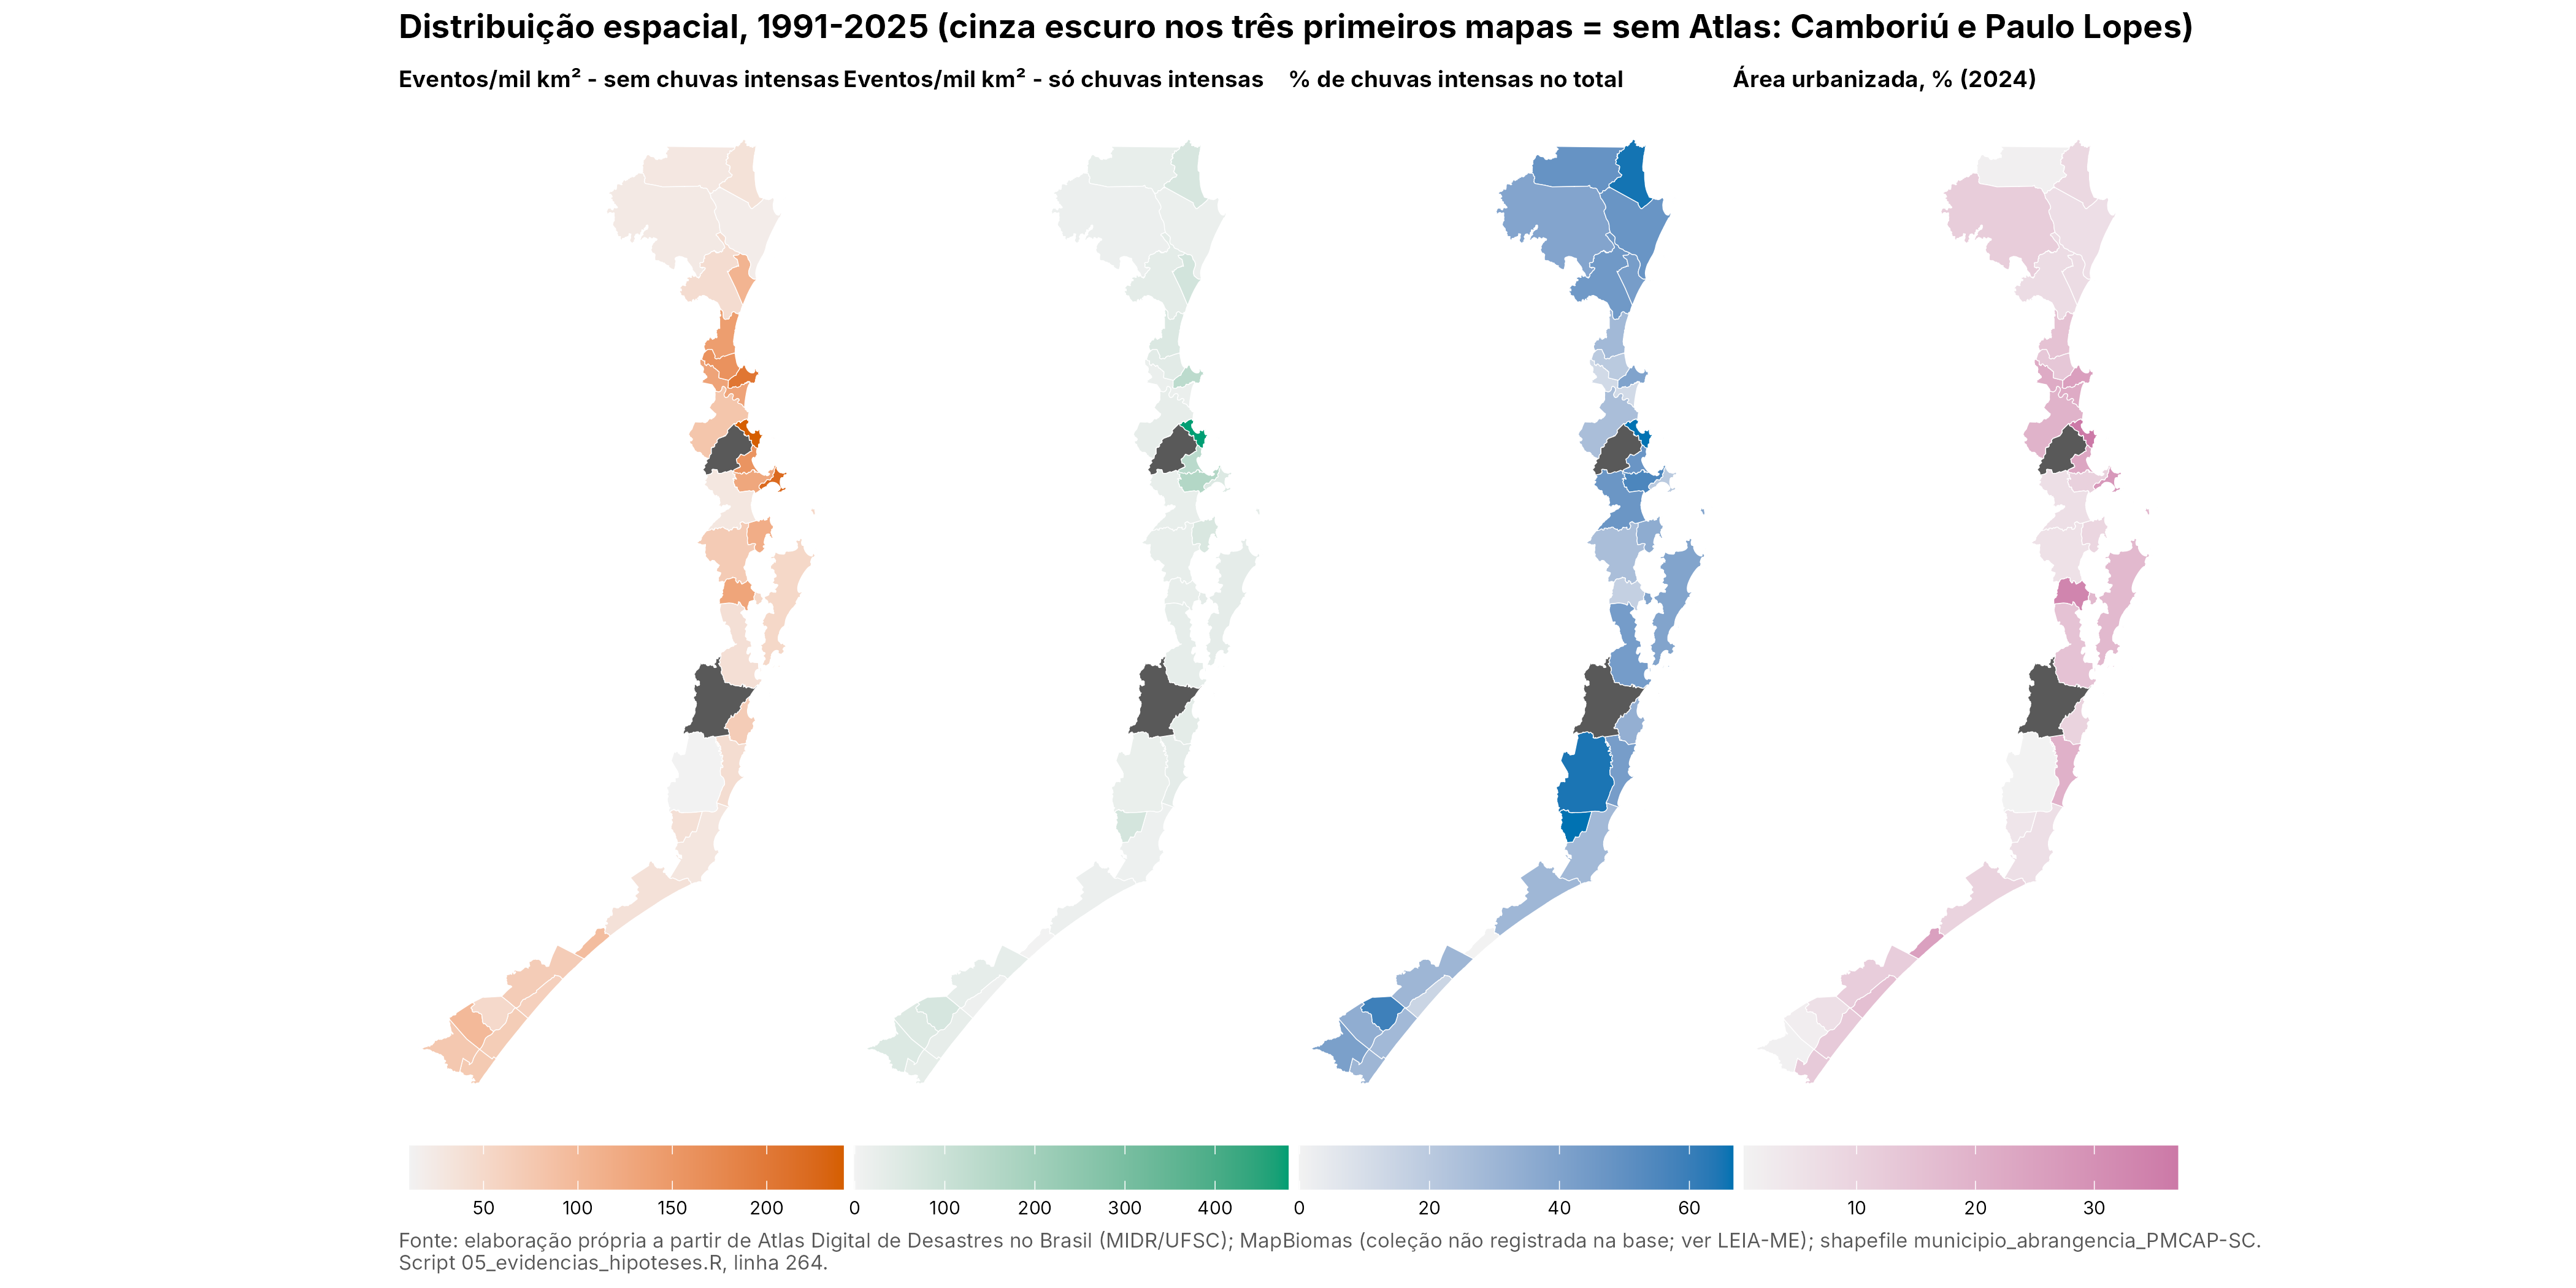
\includegraphics[width=0.9\textwidth]{imagens/aed-D4-mapas-densidade-composicao.png}\\[2mm]
{\small Fonte: Elaborado pela autora (D10).}
\end{figure}

% ---------------------------------------------------------------------
\section{Síntese e limitações}
\label{sec:aed-sintese}

Três conclusões descritivas orientam a modelagem. Primeiro, a resposta depende da versão escolhida: o total cresce muito, mas sem Chuvas Intensas quase não muda, e a composição das tipologias mudou depois de 2013. Segundo, a chuva mensal da reanálise não mostra tendência no período, então o aumento dos registros não acompanha, nessa escala, o aumento da chuva. Terceiro, o uso da terra varia quase só entre municípios e se mistura com a geografia, de modo que ele descreve diferenças entre lugares, e não mudanças no tempo.

As limitações são as seguintes. A chuva vem de reanálise mensal em grade de 0,25°, sem comparação com estações do INMET ou da ANA. A série de desastres tem 35 pontos anuais e uma quebra de classificação em 2013, o que fere as premissas de testes como o de Mann-Kendall, razão pela qual ele é usado apenas para descrever. As séries do MapBiomas têm cobertura incompleta (falta 2025, e a superfície de água cobre 25 municípios), e a coleção usada não está registrada na base consolidada. Os valores de impacto econômico do Atlas estão na unidade original, sem correção monetária, e por isso não foram comparados no tempo (C08). Por fim, o shapefile tem 81 feições e três colunas de código; a junção pela regra do script original fechou os 37 municípios, mas o GDAL corrigiu anéis com orientação inválida sem intervenção.

Os scripts, as 38 tabelas e as 15 figuras que sustentam este capítulo estão no repositório da pesquisa, e cada tabela traz o script e a linha em que foi gerada \pendente{indicar o endereço e a versão do repositório do capítulo 4}.